% \def\bmode{0} % Mode 0 for presentation, mode 1 for a handout with notes, mode 2 for handout without notes
% \if 0\bmode
% \documentclass[smaller]{beamer}
% \else \if 1\bmode
% \immediate\write18{pdflatex -jobname=\jobname-Handout-Notes\space\jobname}
% \documentclass[smaller,handout]{beamer}
% \usepackage{handoutWithNotes}
% \pgfpagesuselayout{2 on 1 with notes}[letterpaper, landscape, border shrink=4mm]
% \else \if 2\bmode
% \immediate\write18{pdflatex -jobname=\jobname-Handout\space\jobname}
% \documentclass[smaller,handout]{beamer}
% \fi
% \fi
% \fi

\documentclass[smaller]{beamer}

% \usepackage[T1]{fontenc} 
% \usepackage{lmodern} 
%\usepackage{etex}
 %\newcommand{\num}{6{} }

% \usetheme[
%   outer/progressbar=foot,
%   outer/numbering=fraction,
%   block=fill,
%   inner/subsectionpage=progressbar
% ]{metropolis}
\usetheme{Madrid}
\useoutertheme[subsection=false]{miniframes} % Alternatively: miniframes, infolines, split
\useinnertheme{circles}
% %\useoutertheme{Frankfurt}
% \usecolortheme{beaver}
% %\useoutertheme{crane}
% %\useoutertheme{metropolis}
\usepackage[backend=biber,style=authoryear,maxcitenames=2,maxbibnames=99,safeinputenc,url=false, eprint=false]{biblatex}
%\addbibresource{bib/references.bib}
% \AtEveryCitekey{\iffootnote{{\tiny}\tiny}{\tiny}}

% %\usepackage{pgfpages}
% %\setbeameroption{hide notes} % Only slides
% %\setbeameroption{show only notes} % Only notes
% %\setbeameroption{hide notes} % Only notes
% %\setbeameroption{show notes on second screen=right} % Both

% % \usepackage[sfdefault]{Fira Sans}

% % \setsansfont[BoldFont={Fira Sans}]{Fira Sans Light}
% % \setmonofont{Fira Mono}

% %\usepackage{fira}
% %\setsansfont{Fira}
% %\setmonofont{Fira Mono}
% % To give a presentation with the Skim reader (http://skim-app.sourceforge.net) on OSX so
% % that you see the notes on your laptop and the slides on the projector, do the following:
% % 
% % 1. Generate just the presentation (hide notes) and save to slides.pdf
% % 2. Generate onlt the notes (show only nodes) and save to notes.pdf
% % 3. With Skim open both slides.pdf and notes.pdf
% % 4. Click on slides.pdf to bring it to front.
% % 5. In Skim, under "View -> Presentation Option -> Synhcronized Noted Document"
% %    select notes.pdf.
% % 6. Now as you move around in slides.pdf the notes.pdf file will follow you.
% % 7. Arrange windows so that notes.pdf is in full screen mode on your laptop
% %    and slides.pdf is in presentation mode on the projector.

% % Give a slight yellow tint to the notes page
% \setbeamertemplate{note page}{\pagecolor{yellow!5}\insertnote}\usepackage{palatino}

% %\usetheme{metropolis}
% %\usecolortheme{beaver}
 \usepackage{tipa}
% \usepackage{enumerate}
% \definecolor{darkcandyapplered}{HTML}{A40000}
% \definecolor{lightcandyapplered}{HTML}{e74c3c}

% %\setbeamercolor{title}{fg=darkcandyapplered}

% \definecolor{UBCblue}{rgb}{0.04706, 0.13725, 0.26667} % UBC Blue (primary)
% \definecolor{UBCgrey}{rgb}{0.3686, 0.5255, 0.6235} % UBC Grey (secondary)

% % \setbeamercolor{palette primary}{bg=darkcandyapplered,fg=white}
% % \setbeamercolor{palette secondary}{bg=darkcandyapplered,fg=white}
% % \setbeamercolor{palette tertiary}{bg=darkcandyapplered,fg=white}
% % \setbeamercolor{palette quaternary}{bg=darkcandyapplered,fg=white}
% % \setbeamercolor{structure}{fg=darkcandyapplered} % itemize, enumerate, etc
% % \setbeamercolor{section in toc}{fg=darkcandyapplered} % TOC sections
% % \setbeamercolor{frametitle}{fg=darkcandyapplered,bg=white} % TOC sections
% % \setbeamercolor{title in head/foot}{bg=white,fg=white} % TOC sections
% % \setbeamercolor{button}{fg=darkcandyapplered} % TOC sections

% % % Override palette coloring with secondary
% % \setbeamercolor{subsection in head/foot}{bg=lightcandyapplered,fg=white}

%\usecolortheme{crane}
% \makeatletter
% \setbeamertemplate{headline}{%
%   \begin{beamercolorbox}[colsep=1.5pt]{upper separation line head}
%   \end{beamercolorbox}
%   \begin{beamercolorbox}{section in head/foot}
%     \vskip1pt\insertsectionnavigationhorizontal{\paperwidth}{}{}\vskip1pt
%   \end{beamercolorbox}%
%   \ifbeamer@theme@subsection%
%     \begin{beamercolorbox}[colsep=1.5pt]{middle separation line head}
%     \end{beamercolorbox}
%     \begin{beamercolorbox}[ht=2.5ex,dp=1.125ex,%
%       leftskip=.3cm,rightskip=.3cm plus1fil]{subsection in head/foot}
%       \usebeamerfont{subsection in head/foot}\insertsubsectionhead
%     \end{beamercolorbox}%
%   \fi%
%   \begin{beamercolorbox}[colsep=1.5pt]{lower separation line head}
%   \end{beamercolorbox}
% }
% \makeatother

% Reduce size of frame box
\setbeamertemplate{frametitle}{%
    \nointerlineskip%
    \begin{beamercolorbox}[wd=\paperwidth,ht=2.0ex,dp=0.6ex]{frametitle}
        \hspace*{1ex}\insertframetitle%
    \end{beamercolorbox}%
}


%\setbeamercolor{frametitle}{bg=darkcandyapplered!80!black!90!white}
%\setbeamertemplate{frametitle}{\bf\insertframetitle}

%\setbeamercolor{footnote mark}{fg=darkcandyapplered}
%\setbeamercolor{footnote}{fg=darkcandyapplered!70}
%\Raggedbottom
%\setbeamerfont{page number in head/foot}{size=\tiny}
%\usepackage[tracking]{microtype}


% %\usepackage[sc,osf]{mathpazo}   % With old-style figures and real smallcaps.
% %\linespread{1.025}              % Palatino leads a little more leading

% % Euler for math and numbers
% %\usepackage[euler-digits,small]{eulervm}
% %\AtBeginDocument{\renewcommand{\hbar}{\hslash}}
\usepackage{graphicx,multirow,booktabs}


% %\mode<presentation> { \setbeamercovered{transparent} }

\setbeamertemplate{navigation symbols}{}
\makeatletter
\def\beamerorig@set@color{%
  \pdfliteral{\current@color}%
  \aftergroup\reset@color
}
\def\beamerorig@reset@color{\pdfliteral{\current@color}}
\makeatother


% %=== GRAPHICS PATH ===========
\graphicspath{{./images/}}
% % Marginpar width
% %Marginpar width
% %\setlength{\marginparsep}{.02in}


% %% Captions
% % \usepackage{caption}
% % \captionsetup{
% %   labelsep=quad,
% %   justification=raggedright,
% %   labelfont=sc
% % }

% \setbeamerfont{caption}{size=\footnotesize}
% \setbeamercolor{caption name}{fg=darkcandyapplered}

% %AMS-TeX packages

\usepackage{amssymb,amsmath,amsthm,mathtools}
\DeclareMathOperator*{\argmax}{arg\,max}
\DeclareMathOperator*{\argmin}{arg\,min}
\usepackage{bm}
% \usepackage{color}

% %https://tex.stackexchange.com/a/31370/2269
% \usepackage{mathtools,cancel}

% \renewcommand{\CancelColor}{\color{red}} %change cancel color to red

% \makeatletter
% \let\my@cancelto\cancelto %copy over the original cancelto command
% \newcommand<>{\cancelto}[2]{\alt#3{\my@cancelto{#1}{#2}}{\mathrlap{#2}\phantom{\my@cancelto{#1}{#2}}}}
% % redefine the cancelto command, using \phantom to assure that the
% % result doesn't wiggle up and down with and without the arrow
% \makeatother


% %\usepackage{comment}
% %\usepackage{hyperref,enumerate}
% \usepackage{minitoc,array}

% \definecolor{slblue}{rgb}{0,.3,.62}
% % \hypersetup{
% %     colorlinks,%
% %     citecolor=blue,%
% %     filecolor=blue,%
% %     linkcolor=blue,
% %     urlcolor=slblue
% % }

% \usepackage{epstopdf}
% \epstopdfDeclareGraphicsRule{.gif}{png}{.png}{convert gif:#1 png:\OutputFile}
% \AppendGraphicsExtensions{.gif}

% %\usepackage{listings}

% %%% TIKZ
% \usepackage{forest}
\usepackage{tikz}
\usepackage{pgfplots}
\usepackage{pgfplotstable}
%\usepackage{pgfgantt}
\pgfplotsset{compat=newest}

\usetikzlibrary{fit,arrows,shapes,positioning,shapes.geometric}
\usetikzlibrary{decorations.markings}
\usetikzlibrary{shadows,automata}
\usetikzlibrary{patterns}
\usetikzlibrary{trees,mindmap,backgrounds}
%\usetikzlibrary{circuits.ee.IEC}
\usetikzlibrary{decorations.text}
% % For Sagnac Picture
% \usetikzlibrary{%
%     decorations.pathreplacing,%
%     decorations.pathmorphing%
% }
% \tikzset{no shadows/.style={general shadow/.style=}}
% %
% %\usepackage{paralist}

% \tikzset{
%   font=\Large\sffamily\bfseries,
%   red arrow/.style={
%     midway,red,sloped,fill, minimum height=3cm, single arrow, single arrow head extend=.5cm, single arrow head indent=.25cm,xscale=0.3,yscale=0.15,
%     allow upside down
%   },
%   black arrow/.style 2 args={-stealth, shorten >=#1, shorten <=#2},
%   black arrow/.default={1mm}{1mm},
%   tree box/.style={draw, rounded corners, inner sep=1em},
%   node box/.style={white, draw=black, text=black, rectangle, rounded corners},
% }

% %%% FORMAT PYTHON CODE
% %\usepackage{listings}
% % Default fixed font does not support bold face
% \DeclareFixedFont{\ttb}{T1}{txtt}{bx}{n}{8} % for bold
% \DeclareFixedFont{\ttm}{T1}{txtt}{m}{n}{8}  % for normal

% % Custom colors
% \definecolor{deepblue}{rgb}{0,0,0.5}
% \definecolor{deepred}{rgb}{0.6,0,0}
% \definecolor{deepgreen}{rgb}{0,0.5,0}

% %\usepackage{animate}

% % Python style for highlighting
% % \newcommand\pythonstyle{\lstset{
% % language=Python,
% % basicstyle=\footnotesize\ttm,
% % otherkeywords={self},             % Add keywords here
% % keywordstyle=\footnotesize\ttb\color{deepblue},
% % emph={MyClass,__init__},          % Custom highlighting
% % emphstyle=\footnotesize\ttb\color{deepred},    % Custom highlighting style
% % stringstyle=\color{deepgreen},
% % frame=tb,                         % Any extra options here
%     % showstringspaces=false            % 
% % }}

% % % Python environment
% % \lstnewenvironment{python}[1][]
% % {
% % \pythonstyle
% % \lstset{#1}
% % }
% % {}

% % % Python for external files
% % \newcommand\pythonexternal[2][]{{
% % \pythonstyle
% % \lstinputlisting[#1]{#2}}}

% % Python for inline
% % 
% % \newcommand\pythoninline[1]{{\pythonstyle\lstinline!#1!}}

% %\usepackage{algorithm2e}

\newcommand{\eps}{\epsilon}
\newcommand{\bX}{\mb X}
\newcommand{\by}{\mb y}
\newcommand{\bbe}{\bm\beta}
\newcommand{\beps}{\bm\epsilon}
\newcommand{\bY}{\mb Y}

\newcommand{\osn}{\oldstylenums}
\newcommand{\dg}{^{\circ}}
\newcommand{\lt}{\left}
\newcommand{\rt}{\right}
\newcommand{\pt}{\phantom}
\newcommand{\tf}{\therefore}
\newcommand{\?}{\stackrel{?}{=}}
\newcommand{\fr}{\frac}
\newcommand{\dfr}{\dfrac}
\newcommand{\ul}{\underline}
\newcommand{\tn}{\tabularnewline}
\newcommand{\nl}{\newline}
\newcommand\relph[1]{\mathrel{\phantom{#1}}}
\newcommand{\cm}{\checkmark}
\newcommand{\ol}{\overline}
\newcommand{\rd}{\color{red}}
\newcommand{\bl}{\color{blue}}
\newcommand{\pl}{\color{purple}}
\newcommand{\og}{\color{orange!90!black}}
\newcommand{\gr}{\color{green!40!black}}
\newcommand{\dca}{\color{darkcandyapplered}}
\newcommand{\nin}{\noindent}
\newcommand*\circled[1]{\tikz[baseline=(char.base)]{
            \node[shape=circle,draw,thick,inner sep=1pt] (char) {\small #1};}}

\newcommand{\bc}{\begin{compactenum}[\quad--]}
\newcommand{\ec}{\end{compactenum}}

\newcommand{\p}{\partial}
\newcommand{\pd}[2]{\frac{\partial{#1}}{\partial{#2}}}
\newcommand{\dpd}[2]{\dfrac{\partial{#1}}{\partial{#2}}}
\newcommand{\pdd}[2]{\frac{\partial^2{#1}}{\partial{#2}^2}}
\newcommand{\pde}[3]{\frac{\partial^2{#1}}{\partial{#2}\partial{#3}}}
\newcommand{\nmfr}[3]{\Phi\left(\frac{{#1} - {#2}}{#3}\right)}
\newcommand{\Err}{\text{Err}}
\newcommand{\err}{\text{err}}

%\DeclarePairedDelimiter\ceil{\lceil}{\rceil}
%\DeclarePairedDelimiter\floor{\lfloor}{\rfloor}

%%%% GREEK LETTER SHORTCUTS %%%%%
\newcommand{\la}{\lambda}
\renewcommand{\th}{\theta}
\newcommand{\al}{\alpha}
\newcommand{\G}{\Gamma}
\newcommand{\si}{\sigma}
\newcommand{\Si}{\Sigma}


\pgfmathdeclarefunction{poiss}{1}{%
  \pgfmathparse{(#1^x)*exp(-#1)/(x!)}%
  }

\pgfmathdeclarefunction{gauss}{2}{%
  \pgfmathparse{1/(#2*sqrt(2*pi))*exp(-((x-#1)^2)/(2*#2^2))}%
}

\pgfmathdeclarefunction{expo}{2}{%
  \pgfmathparse{#1*exp(-#1*#2)}%
}

\pgfmathdeclarefunction{expocdf}{2}{%
  \pgfmathparse{1 -exp(-#1*#2)}%
}


% \usepackage{pst-plot}

% \usepackage{pstricks-add}
% \usepackage{auto-pst-pdf}   

% \psset{unit = 3}

% \def\target(#1,#2){%
%  {\psset{fillstyle = solid}
%   \rput(#1,#2){%
%     \pscircle[fillcolor = white](0.7,0.7){0.7}
%     \pscircle[fillcolor = blue!60](0.7,0.7){0.5}
%     \pscircle[fillcolor = white](0.7,0.7){0.3}
%     \pscircle[fillcolor = red!80](0.7,0.7){0.1}}}}
% \def\dots[#1](#2,#3){%
%     \psRandom[
%       dotsize = 2pt,
%       randomPoints = 25
%     ](!#2 #1 0.04 sub sub #3 #1 0.04 sub sub)%
%      (!#2 #1 0.04 sub add #3 #1 0.04 sub add)%
%      {\pscircle[linestyle = none](#2,#3){#1}}}


%%%%%%%%%%%%%%%%%%%%%%%%%%%%%%%%%%%%%%%%%%%%%%%%%%%
%%%%%%%%%%%%%%%%%%%%%%%%%%%%%%%%%%%%%%%%%%%%%%%%%%%
\title[CEE 616 1c: Statistics]{ {\normalsize CEE 616:  Big Data  and Machine Learning for Engineers}
  \\ Lecture 1c: Statistics}
\date[\today]{\footnotesize \today}
\author{{\bf Jimi Oke}}
\institute[UMass Amherst]{
%\titlegraphic{\hfill
  \begin{tikzpicture}[baseline=(current bounding box.center)]
    \node[anchor=base] at (-7,0) (its) {
\includegraphics[scale=.3]{UMassEngineering_vert}} ;
  \end{tikzpicture}
  % \hfill\includegraphics[height=1.5cm]{logo}
}

%https://tex.stackexchange.com/questions/55806/mindmap-tikzpicture-in-beamer-reveal-step-by-step
  \tikzset{
    invisible/.style={opacity=0},
    visible on/.style={alt={#1{}{invisible}}},
    alt/.code args={<#1>#2#3}{%
      \alt<#1>{\pgfkeysalso{#2}}{\pgfkeysalso{#3}} % \pgfkeysalso doesn't change the path
    },
  }


% https://tex.stackexchange.com/questions/446468/labels-with-arrows-for-an-equation
% https://tex.stackexchange.com/a/402466/121799
\newcommand{\tikzmark}[3][]{
\ifmmode
\tikz[remember picture,baseline=(#2.base)] \node [inner sep=0pt,#1](#2) {$#3$};
\else
\tikz[remember picture,baseline=(#2.base)] \node [inner sep=0pt,#1](#2) {#3};
\fi
}

% \lstset{language=matlab,
%                 basicstyle=\scriptsize\ttfamily,
%                 keywordstyle=\color{blue}\ttfamily,
%                 stringstyle=\color{blue}\ttfamily,
%                 commentstyle=\color{gray}\ttfamily,
%                 morecomment=[l][\color{gray}]{\#}
%               }


              
\begin{document}

\maketitle

\begin{frame}
  \frametitle{Outline}
  \tableofcontents
\end{frame}


\section{Introduction}
\begin{frame}
  \frametitle{Model fitting}
  \pause At the heart of supervised learning is the process of training/fitting a model by estimating its parameters
  $\bm \theta$ (e.g.\ coefficients in a linear regression model) from a dataset $\mathcal{D}$.
  \pause
  \bigskip
  This is essentially an optimization problem of the form:
  \pause
  \begin{equation}
    \bm{\hat\theta} = \argmin\limits_{\bm\theta}\mathcal{L}(\bm\theta)
  \end{equation}
  \pause
  where:
  \pause
  \begin{itemize}
  \item $\bm{\hat\theta}$ is the point estimate of the true value $\bm\theta$ \pause
  \item $\mathcal{L}(\bm\theta)$ is a \textit{loss} or \textit{objective} function (e.g. negative log-likelihood) 
\end{itemize}


\end{frame}



\begin{frame}
  \frametitle{Loss function}
  \pause

  Generally, the performance of a prediction model is evaluated via a \textbf{loss function} $L(Y,\hat f(X))$, which measures errors between $Y$ and $\hat f(X)$.\\\pause

  \bigskip

  Typical choices of the loss function are the \textbf{\rd squared error} and \textbf{\og absolute error}:
  \pause
  \begin{equation}
    \label{eq:10}
    L(Y,\hat f(X)) =
    \begin{cases}
      \rd (Y - \hat f(X))^2 & \text{\rd squared error} \\
      \og |Y - \hat f(X)|   & \text{\og absolute error}
    \end{cases}
  \end{equation}
  \pause
  In the classification case, where the group/class is estimated directly, the \textbf{\bl 0-1 loss function} is typically used:\pause
  \begin{equation}
    \label{eq:10b}
    L(G,\hat G(X)) = {\bl \mathbb{I}(G \ne \hat G(X)) \quad \text{ (0-1 loss) } }
  \end{equation}
  \pause
  where $G$ is the categorical response variable (class). \\ \pause

  In the probabilistic classification case (e.g.\ logistic regression), the \textbf{\pl deviance} measures information loss due to the estimated model:\pause
  \begin{equation}
    \label{eq:10c}
        L(G,\hat p(X)) = {\pl - 2\sum_{k=1}^K  \mathbb{I}(G = k) \log \hat p_k (X) = -2\log\hat p_G(X) \quad (-2\times\text{log-likelihood}) }
  \end{equation}
\end{frame}


\begin{frame}
  \frametitle{Model assessment and selection}\pause
  % \begin{minipage}[t]{.7\linewidth}
  \begin{description}[widest={withdfds}]
  \item[\bf Selection:] estimation of the performance (training/in-sample/validation/extra-sample error) of different models in
    order to choose the best one\pause
  \item[\bf Assessment:] estimation of prediction/test error of final model on new (unseen) data
  \end{description}\pause
  \bigskip
  
  These tasks require a tripartite split of the dataset:\pause
% \end{minipage}\hfill \pause
% \begin{minipage}[t]{.25\linewidth}
  \begin{figure}[h!]
    \centering
    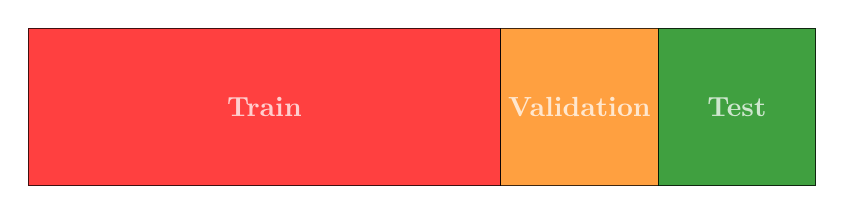
\begin{tikzpicture}
    \draw[fill=red,opacity=.75]     (0,0) rectangle node[white]{\bf Train}  (6,2) ;
    \draw[fill=orange, opacity=.75] (6,0) rectangle node[white]{\bf Validation}  (8,2) ;
    \draw[fill=green!50!black, opacity=.75]  (8,0) rectangle node[white]{\bf Test}  (10,2) ;
  \end{tikzpicture}  
  \caption{Illustration of a 60:20:20 training/validation/test set split for a data set}
  \label{fig:split}
\end{figure}
% \end{minipage}

\end{frame}


  \begin{frame}
   \frametitle{Error estimation methods for model selection}
   \pause
   To select the best of alternative model specifications, we can estimate and compare: \pause
   \begin{itemize}
   \item in-sample errors, $\text{Err}_{in}$ 
   \item extra-sample errors, $\Err_{\tau}$
   \end{itemize}

   \begin{block}{In-sample error estimation approaches} \pause
     \begin{itemize}[<+->]
   \item $C_p$ statistic
   \item Akaike information criterion (AIC)
   \item Bayesian information criterion (BIC)
   \end{itemize}
 \end{block}
 \pause
 
   \begin{block}{Extra-sample error estimation approaches} \pause
   \begin{itemize}[<+->]
   \item Cross-validation (LOOCV, $k$-fold CV)
   \item Bootstrapping and other re-sampling methods  
   \end{itemize}
 \end{block}
   % \pause
   % While these are widely applicable to various contexts, the in-sample error is a
   % viable alternative for model selection. \pause

   % \bigskip
   % We consider three approaches for estimating the in-sample error:\pause
   % \begin{itemize}[<+->]
   % \item $C_p$ statistic
   % \item Akaike information criterion (AIC)
   % \item Bayesian information criterion (BIC)
   % \end{itemize}
   
 \end{frame}

 

\section{MLE}

\begin{frame}
  \frametitle{Point estimates}
  \begin{definition}
    A \textbf{point estimate} of a parameter $\theta$ is a single number that can be regarded as a sensible value for
    $\theta$ and is obtained by computing the value of a suitable statistic from given sample data. \pause The selected
    statistic is the \textbf{point estimator} of $\theta$.
  \end{definition}
  \pause
  \begin{block}{Notation}\pause
    \begin{itemize} 
    \item $\bm{\hat\Theta}$: point estimator (pronounced {\it theta hat}) \pause
    \item $\bm{\hat\theta}$: point estimate\pause
      \begin{equation}
        \label{eq:3}
        \bm{\hat\theta}  = \bm\theta + \text{ estimation error}\pause
      \end{equation}
    \item A hat can be placed on the actual statistic estimated for clarity, e.g. \pause
      \begin{equation*}
        \hat{\mu} = \ol{X}
      \end{equation*}
    \end{itemize}
  \end{block}
\end{frame}

\begin{frame}
  \frametitle{Desired properties of point estimators}
  \begin{block}{Unbiasedness}
    An estimator is \textit{unbiased} if its expected value is equal to the true value of the parameter it estimates:\pause
    \begin{equation}
      \label{eq:1}
      E(\hat\theta) = \theta \pause \quad \text{(if $\hat\theta$ is unbiased)}
    \end{equation}
    \pause
    Thus, the \textbf{\rd bias} is given by:\pause
    \begin{equation}
      \label{eq:2}\rd
     \text{Bias}_{\hat\theta} = \pause  E(\hat\theta) - \theta
    \end{equation}
  \end{block}
  \pause

  \begin{block}{Consistency}\pause
    An estimator is consistent if $\hat\theta \to \theta$ as $n\to \infty$,\pause i.e. the estimation error should decrease with increasing sample size.
  \end{block}

  \pause
  Other properties are: sufficiency and efficiency
\end{frame}

\begin{frame}
  \frametitle{Mean squared error of an estimator}
  \pause

  The mean squared error (MSE) of an estimator is given by:

  \pause

  \begin{equation}
    MSE_{\hat\theta} \pause = \text{Bias}_{\hat\theta}^{2} + \sigma_{\hat\theta}^{2}
  \end{equation}

  \pause

  Recall that the bias of the estimator is given by: \pause

  \begin{equation}
    \label{eq:2}\rd
    \text{Bias}_{\hat\theta} = \pause  E(\hat\theta) - \theta
  \end{equation}
   
\end{frame}

\begin{frame}
  \frametitle{Bias vs. variance}

  \pause

  \begin{center}
    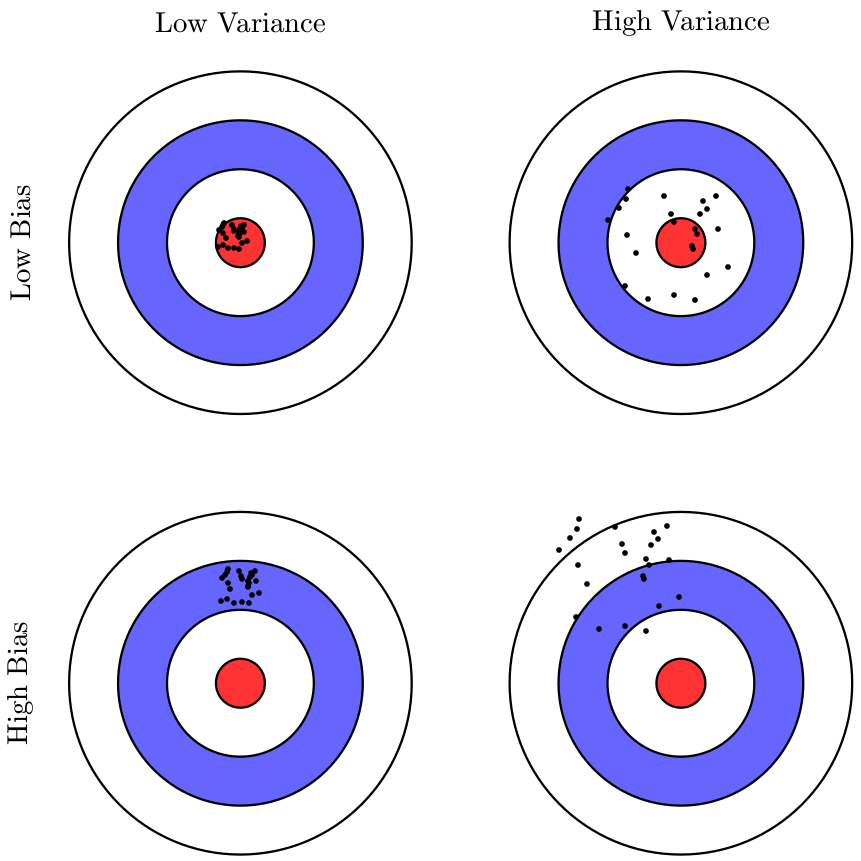
\includegraphics[width=.5\textwidth]{bivar}
  \end{center}
% \begin{pspicture}(3.45,3.45)
%   \target(0.25,0)
%   \target(2.05,0)
%   \target(0.25,1.8)
%   \target(2.05,1.8)
%   \dots[0.12](0.95,1.1)
%   \dots[0.1](0.92,2.53)
%   \dots[0.3](2.5,1.15)
%   \dots[0.3](2.7,2.5)
%   \rput{90}(0.05,0.7){High Bias}
%   \rput{90}(0.05,2.5){Low Bias}
%   \rput(0.95,3.4){Low Variance}
%   \rput(2.75,3.4){High Variance}
% \end{pspicture}

{\footnotesize Image source: \url{https://tex.stackexchange.com/a/307285/2269}}
\end{frame}


\begin{frame}
  \frametitle{ Maximum likelihood estimation (MLE)}
  \pause

  % The  frequentist approach typically seeks a point estimate $\bm{\hat\theta}$. \pause

  % \bigskip

  The most commonly used method for finding $\bm{\hat\theta}$ is \textbf{maximum likelihood estimation} (MLE),
  which holds that the optimal value of $\bm{\hat\theta}$ is that which maximizes the likelihood: \pause
  \begin{equation}
    \bm{\hat\theta}_{\mathrm{mle}} := \argmax_{\bm\theta} p(\mathcal{D}|\bm\theta)
  \end{equation}

  \begin{block}{Likelihood function}
    \pause
    Typically assume observations are sampled independently from the same distribution (\textbf{iid}: independent and identically distributed). Thus:
    \begin{equation}
      p(\mathcal{D}|\bm\theta) = \pause \prod_{n=1}^{N}p(\bm y_n|\bm x_n, \bm\theta)
    \end{equation}
    \pause
    Practically, we \textit{minimize} the \textbf{negative log-likelihood} (NLL), given by: \pause
    \begin{equation}
      \mathsf{NLL}(\bm\theta) := -\log p(\mathcal{D}|\bm\theta)  = -\sum_{n=1}^N\log p(\bm y_n|\bm x_n, \bm\theta)
    \end{equation}
  \end{block}
\end{frame}


\begin{frame}
  \frametitle{Maximum likelihood and least squares}
  \pause
  Based on ordinary least squares assumptions, $Y$ is normally distributed as:\pause
  \begin{equation}
    \bm Y| \bm X \sim \mathcal{N}(\bm X\bm\beta, \sigma^2\bm I)
  \end{equation}
  \pause
  (in matrix notation). \pause
  \bigskip
  Recall the normal/Gaussian density function:\pause
  \begin{equation}
    f_Y(y) = \fr1{\sqrt{2\pi}\sigma}\exp\lt(-\fr1{2\sigma^2}(y - \mu_Y)^2 \rt)
  \end{equation}
  \pause
  The log-likelihood is thus given by:\pause
  \begin{equation}
    \ell(\bm\beta) = -\fr n2\log2\pi -\fr n2\log(\sigma^2) -
    \fr1{2\sigma^2} (\bm Y - \bm{X\beta})^T(\bm Y - \bm{X\beta})
  \end{equation}
  \pause
  Differentiating w.r.t.\ to $\bm\beta$ and setting to zero, we obtain:\pause
  \begin{equation}
    \fr{1}{\sigma^2}(\bm Y - \bm{X\beta})^T{\bm X} = \pause     \fr{1}{2\sigma^2}(\bm Y^T\bm X - \bm\beta^T\bm X^T\bm X) = \pause 0
  \end{equation}
\end{frame}

\begin{frame}
  \frametitle{Maximum likelihood and least squares (cont.)}
  Solving the equation, we obtain:\pause
  \begin{eqnarray}
       \bm Y^T\bm X - \hat{\bm\beta}^T\bm{X}^T\bm{X}  &=& 0 \\ \pause
      \hat{\bm\beta}^T\bm X^T\bm X &=& \bm{Y}^T\bm{X}  \\\pause
      \hat{\bm\beta}^T\bm X^T\bm X (\bm X^T \bm X)^{-1}&=& \bm{Y}^T\bm{X}(\bm X^T \bm X)^{-1}  \\\pause
      \implies\quad \pause \hat{\bm \beta} &=& (\bm X^T \bm X)^{-1}\bm X^T \bm Y
   \end{eqnarray}
  \pause
  Thus, we see that the MLE of $\bm\beta$ is equivalent to its least squares estimate.
%  \pause

  % \begin{alertblock}{Note}
  %   The term that depends on $\bm\beta$ in $\ell$ is the $RSS$.
  % \end{alertblock}
\end{frame}


\begin{frame}
  \frametitle{Empirical risk minimization (ERM)}
  \pause
  This is a generalization of MLE whereby we minimize any average loss function (or expected loss):
  \pause
  \begin{equation}
    \mathcal{L}(\bm\theta) = \fr1N\sum_{n=1}^N\ell(\bm y_n, \bm\theta; \bm x_n)
  \end{equation}

  \pause

  Other point estimation methods include:\pause
  \begin{itemize}
  \item Method of moments (assume empirical moments are theoretical values)\pause
    \item Online/recursive estimation (e.g. moving average)
  \end{itemize}
\end{frame}

\section{Bayes}


\begin{frame}
  \frametitle{Bayes rule for data}
  Given that we  have some \textbf{prior} knowledge of the parameters $\bm\theta$, governed by the distribution $p(\bm\theta)$. \pause
  \bigskip

  The observed data is given by the \textbf{likelihood}: $p(\mathcal{D}|\bm\theta)$.

  
  \pause
  \bigskip
  
  Then, we can obtain the \textbf{posterior} distribution $p(\bm\theta|\mathcal{D})$ via Bayes rule as follows:
  \begin{equation}
    p(\bm\theta|\mathcal{D}) = \pause \fr{p(\mathcal{D}|\bm\theta)p(\bm\theta)}{p(\mathcal{D})}
    = \pause \fr{p(\mathcal{D}|\bm\theta)p(\bm\theta)}{\int p(\mathcal{D}|\bm\theta')p(\bm\theta') d\bm\theta'}
  \end{equation}

  \pause

  where the denominator is called the \textbf{evidence} or \textbf{marginal likelihood} (normalization constant/average
  probability of the data).

  \pause
  \begin{center}
    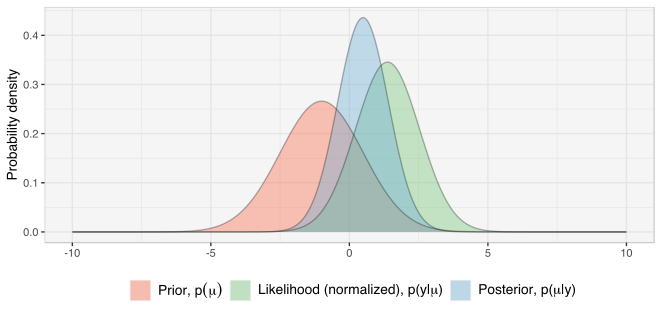
\includegraphics[width=.5\textwidth]{bayes-1.png}
    
    {\scriptsize Source: \url{https://www.boelstad.net/post/bayesian_statistics_introduction/}}
  \end{center}
\end{frame}


\begin{frame}
  \frametitle{Maximum a posterior(i) (MAP) estimation}
  \pause
  From Bayes, we obtain:\pause
  \begin{equation}
     p(\bm\theta|\mathcal{D}) \propto p(\mathcal{D}|\bm\theta)p(\bm\theta)
   \end{equation}

   \pause
   Thus, we can estimate $\bm\hat\theta$ by maximizing the log posterior:\pause
   \begin{equation}
     \bm{\hat\theta} = \argmax_{\bm\theta}\log p(\bm\theta|\mathcal{D}) \pause = \argmax_{\bm\theta}\log [p(\bm\theta|\mathcal{D}) + \log p(\bm\theta)]
   \end{equation}
   \pause
   This approach is called \textbf{MAP estimation}. It gives the most probable value (posterior mode) of $\bm\theta$.

   \pause
   \bigskip
   Other results we can obtain via Bayesian estimation include:\pause
   \begin{itemize}
   \item posterior mean and variance\pause
   \item posterior predictive distribution: \pause
     \begin{equation}
       p(\bm y |\bm x, \mathcal{D}) = \int p(\bm y|\bm x, \bm\theta)p(\bm\theta|\mathcal{D})d\bm\theta       
     \end{equation}
   \end{itemize}
\end{frame}
\section{Error estimation}

\begin{frame}
  \frametitle{Quantifying regression performance}

  \begin{itemize}
  \item Residual sum of squares (RSS):\pause
    \begin{equation}
      RSS(\bm\beta) := \sum_{n=1}^N(y_n - \bm\beta^{T}\bm x_n)^2
    \end{equation}
    \pause
  \item Mean squared error (MSE): \pause
    \begin{equation}
      MSE(\bm\beta) := \fr1N RSS(\bm\beta)
    \end{equation}
    \pause

  \item Root mean squared error (RMSE): \pause
    \begin{equation}
      RMSE(\bm\beta) := \sqrt{MSE(\bm\beta)} = \sqrt{\fr1N  \sum_{n=1}^N(y_n - \bm\beta^{T}\bm x_n)^2}
    \end{equation}
  \end{itemize}
\end{frame}

\begin{frame}
  \frametitle{Quantifying classifier performance}
  \pause
  We can measure how well a classifier performs using the following metrics:\pause
  \begin{itemize}[<+->]
  \item Error rate
  \item Confusion matrix
  \item Receiver operating characteristics (ROC) curve
  \end{itemize}
\end{frame}
\begin{frame}
  \frametitle{Error rates}
  \pause
  \begin{block}{Bayes error rate}\pause
    The Bayes classifier produces the lowest possible prediction error: \pause
    \begin{equation}
     \Err_{\text{Bayes}} = 1 - \mathbb{E}\lt(\max_k \Pr(Y=k|X=x)\rt)
  \end{equation}
\end{block}

  \pause
  \begin{block}{ Error rate}\pause
    This is the ratio of wrong predictions to the total number of predictions:\pause
  \begin{equation}
   \Err =  \fr1n \sum_{i=1}^n \mathbb{I}(y_i \ne \hat y_i)
 \end{equation}\pause
 where:
 \begin{equation}
   \mathbb{I}(y_i \ne \hat y_i) =
   \begin{cases}
     1 & \text{if predicted class for $i$th observation is incorrect} \\
     0 & \text{otherwise}
   \end{cases}
 \end{equation}
\end{block}
\end{frame}

\begin{frame}
  \frametitle{Confusion matrix}
  \pause
  This indicates the correct and incorrect assignments for each class.\pause

  \begin{table}[h!]
    \centering \small
        \caption{Confusion matrix (binary case)}
    \label{tab:conf}
    \begin{tabular}{l l l l l}\toprule
      && \multicolumn{3}{c}{\it Predicted class} \\
      & & $-$ or Null & $+$ or Non-null & Total \\\midrule
      \multirow{2}{*}{\it True class}& $-$ or Null & \bl True Negative (TN) &\rd False Positive (FP) & N \\
                                    & $+$ or Non-null& \rd False Negative (FN) &  \bl True Positive (TP) & P \\\midrule
      & Total & N$^*$ & P$^*$ & \\\bottomrule
    \end{tabular}
  \end{table}
  \pause
  The confusion matrix provides more information than a simple overall error rate.\pause

  \begin{itemize}[<+->]
  \item False positive: Type I error
  \item False negative: Type II error
  \end{itemize}
\end{frame}

\begin{frame}
  \frametitle{Sensitivity and specificity}
  \pause
  \begin{itemize}[<+->]
  \item \textbf{Sensitivity} refers to the ability of the model to correctly classify the positives (non-null) cases (percentage of correct true positives.\\\pause
    Usually, the 50\% threshold is used:\pause
    \begin{equation}
      \Pr(+|X=x) > 0.5
    \end{equation}\pause
    However, to increase the sensitivity of the model to non-null cases, we could reduce the threshold at the cost of the overall error rate.
  \item \textbf{Specificity} is the rate of correctly identifying the null cases (percentage of correct true negatives)
  \end{itemize}
  \pause
  \begin{block}{Summary of performance measures}
    \pause\small
    \begin{tabular}{l l l}
      \bf Name & \bf Definition & \bf Synonym \\\midrule
      False positive rate & FP/N & Type I error, $1-$Specificity \\
      True positive rate & TP/P & 1 - Type II error, power, sensitivity, recall\\
      Positive prediction value & TP/P$^*$ & Precision, $1-$false discovery proportion\\
      Negative prediction value & TN/N$^*$ & \\\bottomrule
    \end{tabular}
  \end{block}
\end{frame}

\begin{frame}
  \frametitle{Receiver operating characteristics (ROC) curve}
  The ROC curve is a plot of the true positive rate (TP/P) vs. false positive rate (FP/N) for different threshold values.\pause
  \begin{figure}[h!]
    \centering
    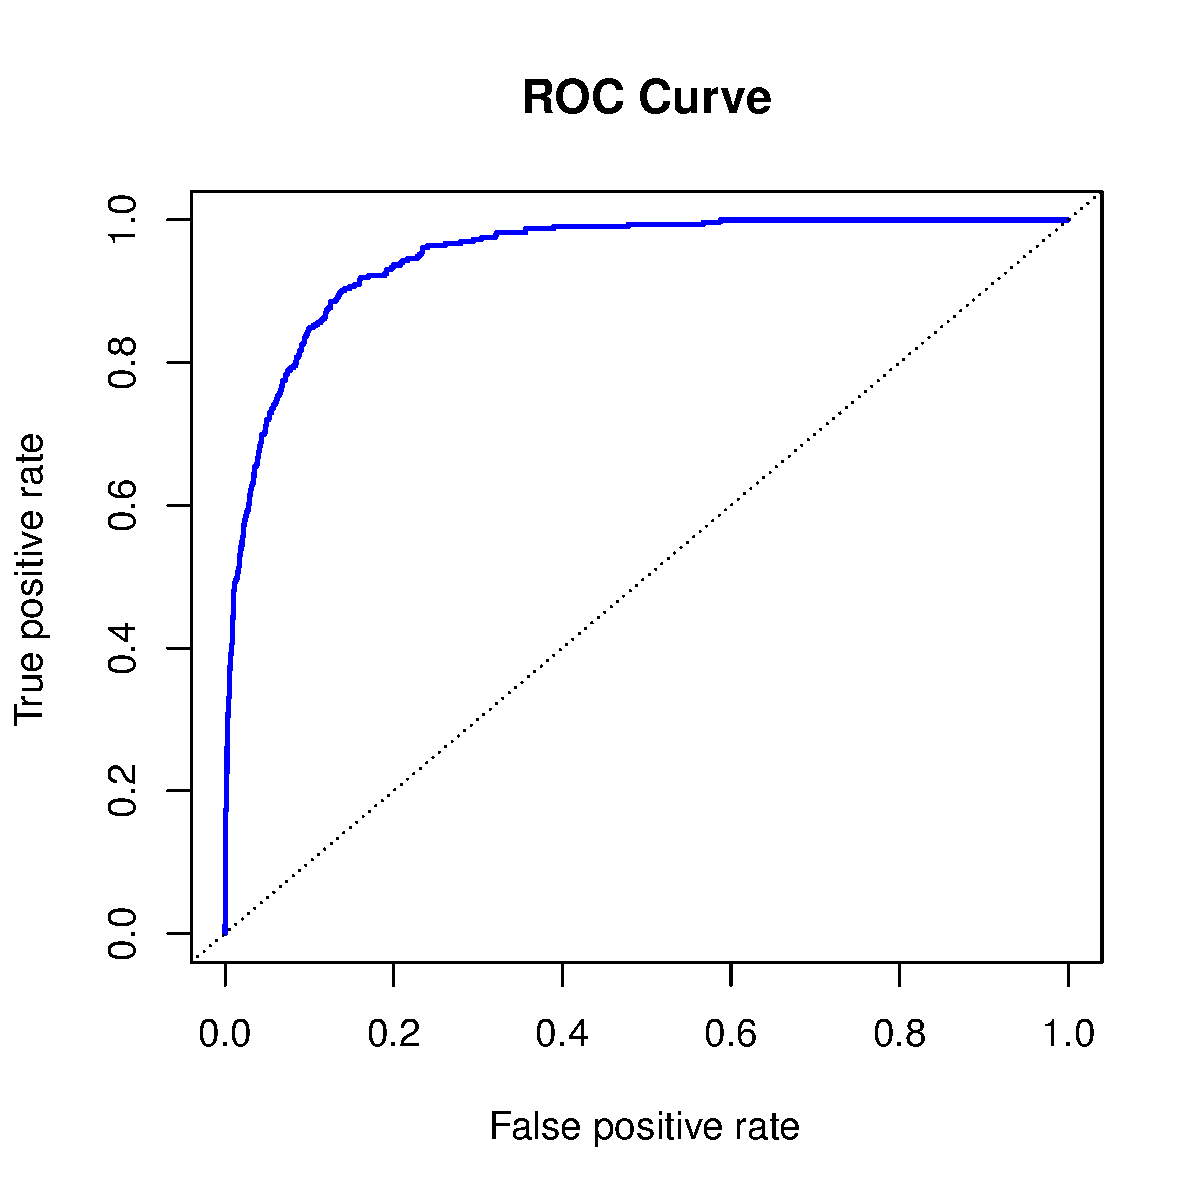
\includegraphics[width=.4\textwidth]{4-8}
    \caption{Example of ROC curve for LDA classifier on Default data. The AUC is 0.95}
  \end{figure}
  \pause
  The \textbf{area under the ROC curve (AUC)} indicates the overall performance of the classifier across different thresholds.\pause
  The maximum AUC value is 1.
\end{frame}

\begin{frame}
  \frametitle{ROC curve (cont.)}
  \pause
  \begin{itemize}[<+->]
  \item The ideal classifier \textit{hugs} the top left of the ROC curve (perfect true positive rate).
  \item While typically used in binary classification, the ROC curve can be extended for multiple class analyses.
\end{itemize}
\pause
\begin{figure}[h!]
  \centering
  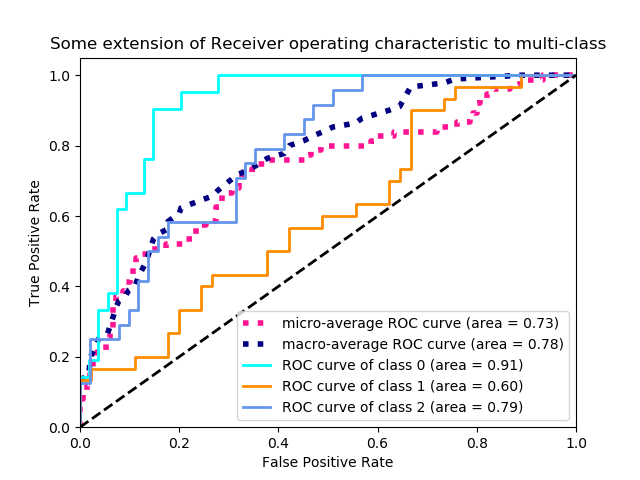
\includegraphics[width=.45\textwidth]{sphx_glr_plot_roc_002}
  \caption{Extension of ROC curve to multiple classes. Source: \url{https://scikit-learn.org/stable/auto_examples/model_selection/plot_roc.html}}
  \label{fig:ext}
\end{figure}
\end{frame}


\begin{frame}
  \frametitle{Error definitions}\pause

  \begin{description}[widest = {tunin},leftmargin=!]
  \item[Test error, $\Err_{\tau}$] prediction error over an \textit{independent} test sample  \pause
  \item[Expected test error, $\Err$] prediction error averaged over all possible test sets (this is usually what is effectively estimated)\pause
  \item[Training error, $\ol{\err}$] average loss over the training sample\pause
  \item[Tuning parameter(s), $\alpha$] this controls the complexity (flexibility) of the model. We typically choose $\alpha$ to minimize error.
  \end{description}
  \pause

  \begin{figure}[h!]
    \centering
    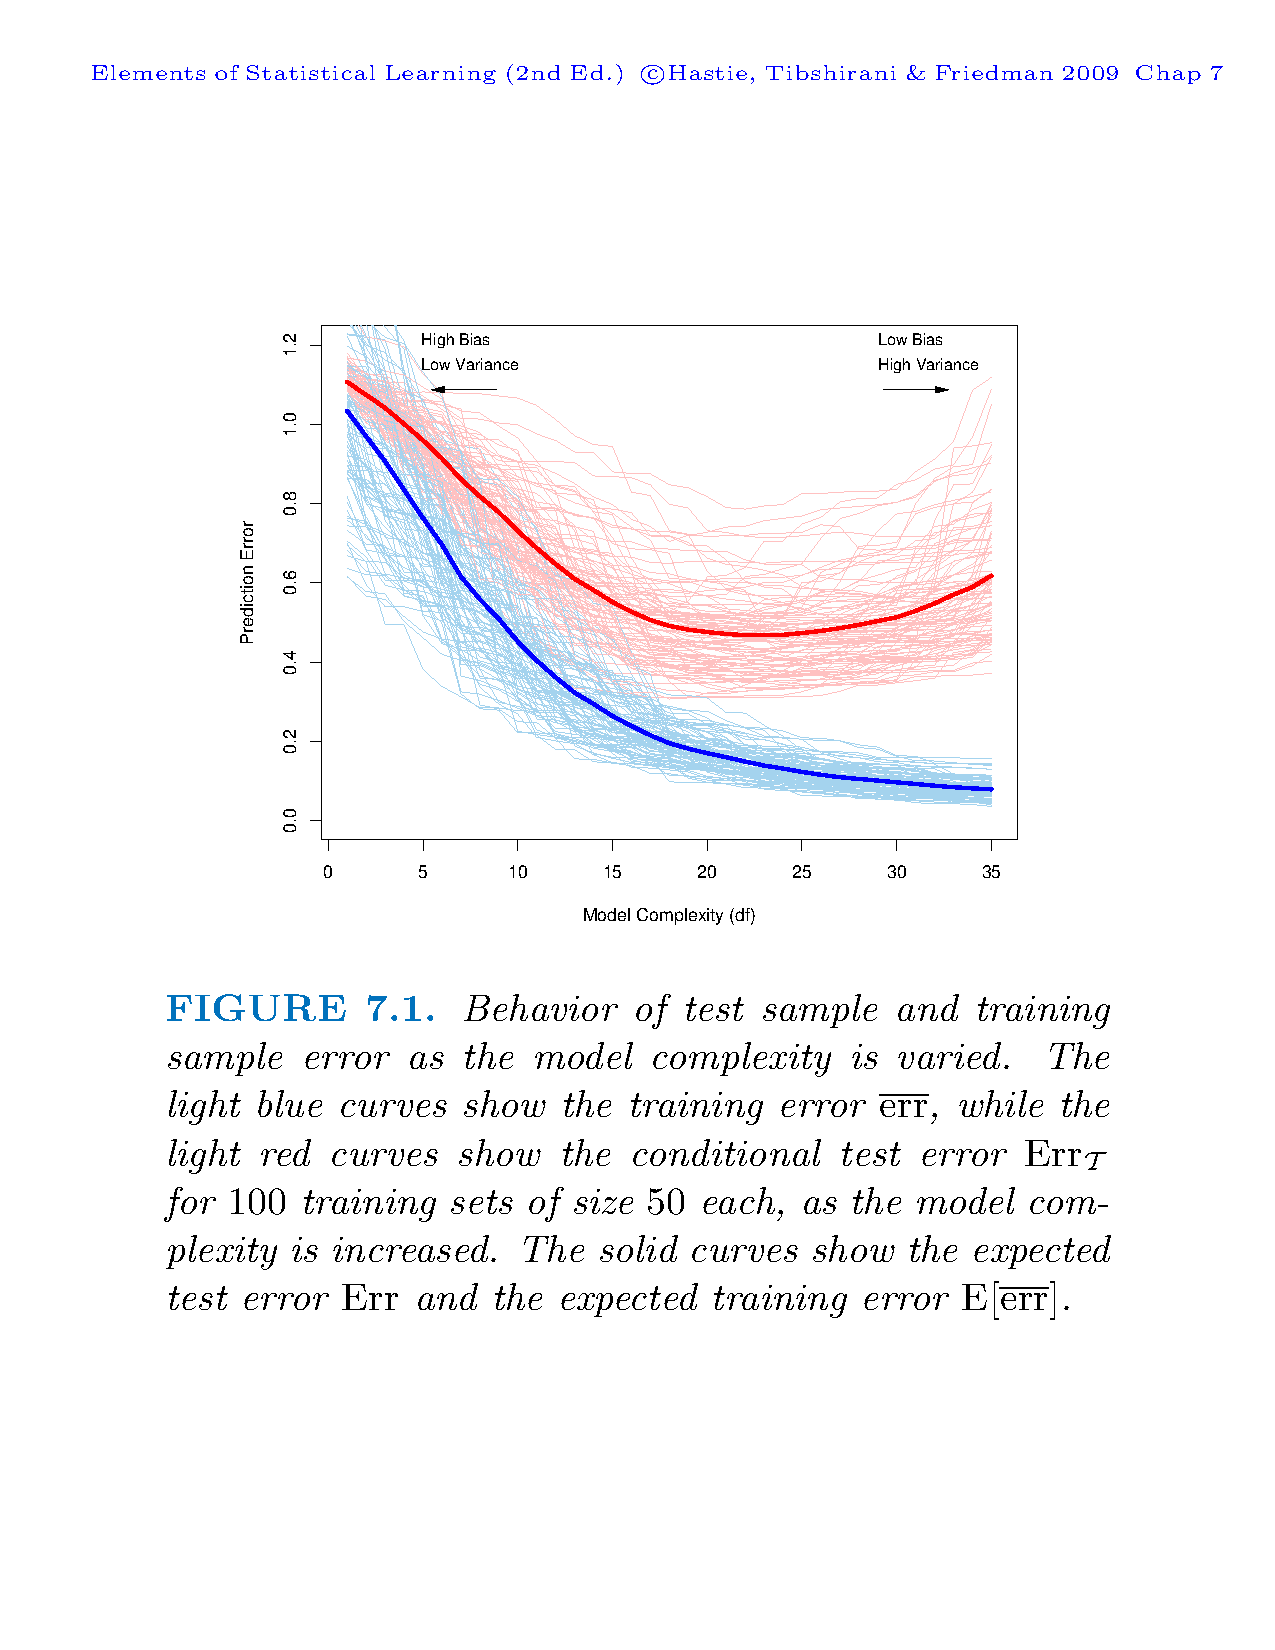
\includegraphics[width=.5\textwidth, trim={2cm 12.2cm 2cm 5cm},clip]{ESL7-1}
    \caption{Test sample and training sample error plotted against model complexity. The light blue curves indicate training error while light red curves indicate test error (for 100 training sets with 50 observations each). The solid curves are the respective averages.}
    \label{fig:mse}
  \end{figure}
\end{frame}




\begin{frame}
  \frametitle{Training error and in-sample error}\pause
  
    \begin{itemize}
    \item The training error {\gr $\ol{\err}$} is the average loss over the training set:\pause
      \begin{equation}
        \label{eq:22}\gr
        \err = \fr1n\sum_{i=1}^n\mathcal{L}(y_i, \hat f(x_i))
      \end{equation}
\pause
    \item $\ol{\err}$  underestimates  $\Err_\tau$. We refer to this as \textit{optimism}
\pause
    \item To compute the optimism in practical terms, we consider the difference between $\ol{\err}$ and the \textbf{in-sample error}
\pause
    \item The \textbf{\pl in-sample error} is the average loss based on new responses generated at each of the $n$ training points:\pause
      \begin{equation}
        \label{eq:6}\pl
        \Err_{in} = \fr1N\sum_{i=1}^N\mathbb{E}_{Y^0}[\mathcal{L}(Y_i^0, \hat f(x_i))|\tau]
      \end{equation}
  \end{itemize}
\end{frame}

\begin{frame}
  \frametitle{Test error}
  \pause

\begin{itemize} 

  \item The \textbf{test} (or generalization) \textbf{error} is the expected error (as defined by the given loss function) over an independent test set $(X, Y)$,
    using a model estimated over a training set $\tau$:\pause
    \begin{equation}
      \Err_\tau = \mathbb{E}[\mathcal{L}(Y, \hat f(X))|\tau]
    \end{equation}
    \pause
    
    \begin{itemize}
    \item When evaluated over a new test data point $(X^{0},Y^{0})$, this quantity is also called the \textbf{\bl extra-sample error}
      \pause
      \begin{equation}\bl
        \label{eq:20}
        \Err_\tau = \pause \mathbb{E}_{X^0,Y^0}[\mathcal{L}(Y^0, \hat f(X^0))|\tau]
      \end{equation}
    \end{itemize}
  \pause
  \item  The \textbf{\rd expected test error} is the average generalization error across different training sets (this quantity is what is typically estimated)
    \pause
    \begin{equation}
      \label{eq:21}\rd
      \Err \pause  = \mathbb{E}(\Err_\tau)  \pause = \mathbb{E}_{\tau}\pause \mathbb{E}_{X^0,Y^0}[\mathcal{L}(Y^0, \hat f(X^0))|\tau]
    \end{equation}
  \end{itemize}
%

\end{frame}




\section{In-sample error}

 
\begin{frame}
  \frametitle{Optimism}
  \pause
  We define \textbf{\rd optimism} as difference between in-sample error and training error:
  \begin{equation}
    \label{eq:7}\rd
    \text{op} = \Err_{in} - \ol{\err}
  \end{equation}
  \pause
  \begin{itemize}
  \item This value is positive as $\ol{\err}$ is an underestimate of $\Err_{in}$
\end{itemize}
  \pause
  \bigskip

  The \textbf{expected optimism} (what is usually estimated) is then:\pause
  \begin{equation}
    \label{eq:8}
    \omega = E_{\bm y}(\text{op})
  \end{equation}
  \pause
  
  For the more widely used loss functions, the average optimism can be generalized by:
  \pause
  \begin{equation}
    \label{eq:9}\bl
    \omega =  \fr2n\sum_{i=1}^n\text{Cov}(\hat y_i, y_i)
  \end{equation}
  \pause
  
  As a model tends toward overfitting, $\text{Cov}(\hat y_i, y_i)$ will increase, and thus will the
  expected optimism $\omega$.
\end{frame}

\begin{frame}
  \frametitle{Expected in-sample error}\pause
  Substituting {\bl \eqref{eq:9}} in {\rd \eqref{eq:7}}, we obtain:\pause
  \begin{equation}
    \label{eq:10}
     E_{\bm y}(\Err_{in}) = \pause E_{\bm y}(\ol\err) + \pause  \fr2n\sum_{i=1}^n\text{Cov}(\hat y_i, y_i)
   \end{equation}
   \pause
   In a linear regression with $d$ inputs, the variance ($\sigma^2$) is constant across all observations. Thus:
   \pause
   \begin{equation}
     \sum_{i=1}^n\text{Cov}(\hat y_i, y_i) = d\sigma^2
   \end{equation}
   \pause
   We can then express the \textbf{\rd expected in-sample error} as:\pause
   \begin{equation}\rd
     E_{\bm y}(\Err_{in}) = \pause E_{\bm y}(\ol\err) + \fr{2d}{n}\sigma^2
   \end{equation}
   \pause

   \note[item]{Optimism is directly proportional to the number of inputs $d$}
   \note[item]{And inversely proportional to sample size $n$}

   Generally, the in-sample error estimate is given by:\pause
   \begin{equation}
     \widehat{\Err}_{in} = \ol\err + \hat\omega
   \end{equation}
 \end{frame}



 \begin{frame}
   \frametitle{$C_p$ statistic}
   \pause
   Recall the general form of the in-sample error estimate:\pause
   \begin{equation}\rd
     E_{\bm y}(\Err_{in}) = \pause E_{\bm y}(\ol\err) + \fr{2d}{n}\sigma^2
   \end{equation}
   \pause

   Using a squared error loss function, the {\bl $C_p$ estimate}\footnote{\bl Also known as ``Mallows's $C_p$ after English statistician, Colin Lingwood Mallows} is then given by:\pause
   \begin{equation}\bl
     C_p = MSE + \fr{2d}{n}\hat\sigma^2 = \pause  \fr1n\lt(RSS + 2 d\hat\sigma^2\rt)
   \end{equation}
   \pause
   The noise variance estimate $\hat\sigma^2$ is estimated using the full model containing all predictors
   $\mathcal{M}_p$:\pause
   \begin{equation}
     \hat\sigma^2 = \fr{1}{n-p-1} RSS_p
   \end{equation}
   where $RSS_p$ denotes the $RSS$ computed from the full model.
 \end{frame}

 \begin{frame}
   \frametitle{$C_p$ in practice}
   \pause
   \begin{itemize}[<+->]
   \item In essence, the $C_p$ adds a penalty term (linear in the number of inputs/features $d$) to adjust the understimate of the training error ($MSE$).\\
     
   \item If $\hat\sigma^2$ is an unbiased estimate of $\sigma^2$, then $C_p$ is an unbiased estimate of the test error.\\
     
   \item In choosing the best model from a subset using $C_p$, the optimal $C_p$ is the smallest value.
   \end{itemize}
 \end{frame}
 
\begin{frame}
  \frametitle{Akaike information criterion (AIC)}
  \pause
  The Akaike information criterion\footnote{\bl Proposed by Japanese statistician, Hirotugu Akaike (d.\ 2009)}
  is defined using a {\rd negative log-likelihood loss function}, where\pause
  \begin{equation}
    \widehat\Err_{in} = {\rd -2\mathbb{E}[\log\Pr_{\hat\theta}(Y)]} \pause \approx -\fr2n \mathbb{E}[{\pl \ell^{*}}] + 2\fr d n
  \end{equation}
  Definitions:\pause
  \begin{eqnarray*}
    \Pr_{\theta}(Y) &=&\text{ family of densities for $Y$, containing true density}\\\pause
    \hat\theta &=& \text{ maximum-likelihood estimate of $\theta$ (optimal value)}\\\pause
    \Pr_{\hat\theta}(Y) &=& \text{ estimate of true density of $Y$} \\\pause
    \pl \ell^{*} &\pl=& \pl \sum_{i=1}^n \log \Pr_{\hat\theta}(y_i) \quad \text{ (maximized log-likelihood)}
  \end{eqnarray*}
  \pause
  \note[item]{The asymptotically optimal property of maximum likelihood estimation (MLE), i.e.\ as $n\to \infty$,
  the parameter that maximizes the [log]-likelihood gives the lowest error.}
\end{frame}


\begin{frame}
  \frametitle{AIC for Gaussian model}\pause
  We can write the maximized log-likelihood in the Gaussian case as:\pause
  \begin{eqnarray}
    \ell^{*} &=& -\fr n2\log2\pi -\fr n2\log(\hat\sigma^2) -
    \fr1{2\hat\sigma^2} (\bm Y - \bm{X\hat\beta})^T(\bm Y - \bm{X\hat\beta}) \\\pause
    &=& -\fr n2\log2\pi -\fr n2\log(\hat\sigma^2) -\fr1{2\hat\sigma^2} RSS
   \end{eqnarray}
  \pause
  Recall the in-sample error estimate for log-likelihood loss:
    \begin{equation}
    \widehat\Err_{in}  \approx -\fr2n \mathbb{E}[\ell^{*}] + 2\fr d n
  \end{equation}
  \pause
  Substituting for $\text{loglik}$ and dropping the constant terms, we obtain the {\rd AIC}:\pause
  \begin{eqnarray}
      \text{AIC} &=& -\fr2n \lt( -\fr{1}{2\hat\sigma^2}RSS\rt) + 2 \fr dn\\\pause
      &=& \fr{RSS}{n\hat\sigma^2} + \fr{2d}{n} \\\pause
      &=& \rd \fr{1}{n\hat\sigma^2}(RSS + 2d\hat\sigma^2)
   \end{eqnarray}
\end{frame}

\begin{frame}
  \frametitle{AIC in model selection}
  \pause
  \begin{itemize}[<+->]
  \item For the Gaussian model (normally distributed responses), the AIC statistic is equivalent to $C_p$.
  \item The best model in a subset will have the lowest AIC
  \end{itemize}
\end{frame}
\begin{frame}
  \frametitle{Bayesian information criterion (BIC)}
  The BIC is given by:\pause
  \begin{equation}
    \text{BIC} = -2 \cdot \text{loglik} + d \cdot \log n
  \end{equation}
  \pause
  
  Under the Gaussian model, the BIC is proportional to AIC:\pause
  \begin{equation}
    \label{eq:14}
    \text{BIC} = \fr{1}{n\hat\sigma^2}\lt(RSS + d\hat\sigma^2\cdot \log n\rt)
  \end{equation}
\end{frame}


\section{Cross-validation}

\begin{frame}
  \frametitle{Cross-validation}
  \pause

  Cross-validation provides approaches for extra-sample error estimation\pause
  \begin{itemize}
  \item Used for model selection
    \pause
  \item More practically, in grid searches or other methods for hyperparameter tuning
  \end{itemize}
  \pause


  \begin{center}
    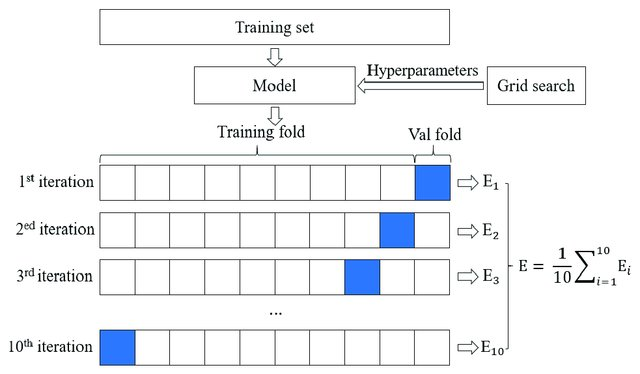
\includegraphics[width=.6\textwidth]{kfold.png}

    {\scriptsize Source: \url{https://www.mdpi.com/1996-1944/14/12/3143}}
  \end{center}

  \pause
  We consider 3 approaches:\pause
  \begin{itemize} 
  \item Validation set approach \pause
  \item Leave-one-out cross-validation\pause
  \item $k$-fold cross-validation 
  \end{itemize}
\end{frame}


\begin{frame}
  \frametitle{Validation set approach}
  \pause
  This simplistic method involves randomly splitting the data into a \textit{training set} and a \textit{validation set}.\pause

  \begin{itemize}[<+->]
  \item This randomness leads to high variability in test error estimation
  \item There is no ``best'' training/validation split ratio. \\ \pause
    \quad Examples: 50:50, 60:40, 75:25, 80:20.
  \item Error from validation set may be an overestimate as it is a subset of all observations
  \end{itemize}
  \pause

  \begin{figure}[h!]
    \centering
    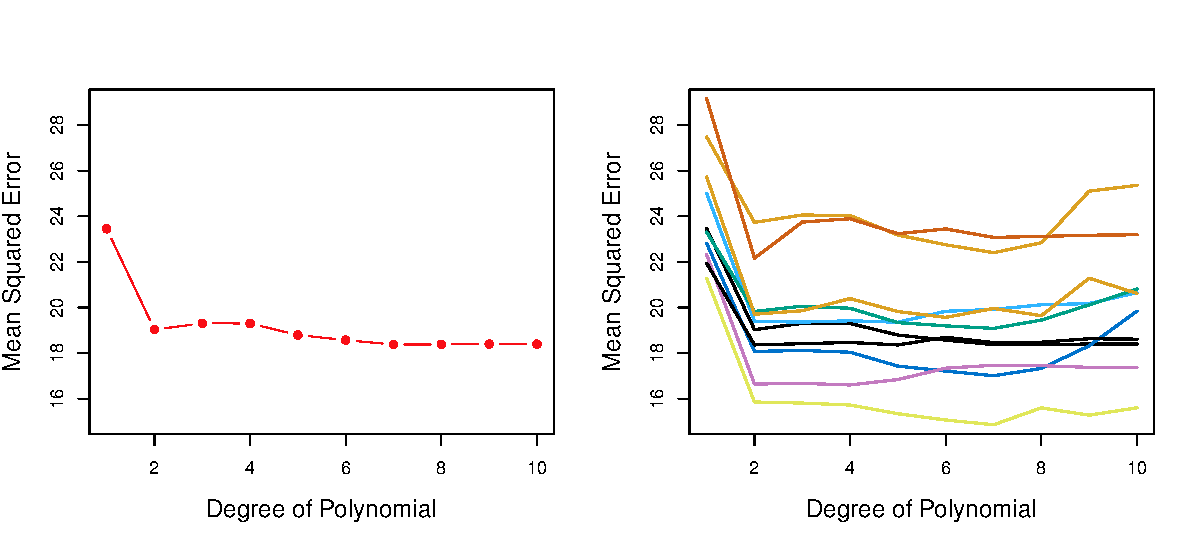
\includegraphics[width=.6\textwidth]{5-2}
    \caption{Example of MSE estimated from the validation set for varying levels of model complexity. (L) Single split. (R) Various random splits.
    There is high variability in the estimates.}
    \label{fig:valset}
  \end{figure}
\end{frame}


\begin{frame}
  \frametitle{Leave-One-Out Cross-Validation (LOOCV)}
  \begin{enumerate}[<+->]
  \item Create a test set with a single observation $(x_1,y_1)$
  \item Estimate the model based on the remaining $n-1$ observations
  \item Compute error in prediction on the single observation test set
    \begin{equation}
      \label{eq:12}\rd
      MSE_i = (y_i - \hat y_i)^2
    \end{equation}    
  \item Repeat steps 1-3 successively using each of the other observations as the test set $(x_2,y_2), \ldots, (x_n,y_n)$
  \item Compute the LOOCV estimate for the test $MSE$:
    \begin{equation}
      \label{eq:11}\rd
      CV_{(n)} = \fr1n\sum_{i=1}^n MSE_i
    \end{equation}
  \end{enumerate}
\end{frame}

\begin{frame}
  \frametitle{Advantages of LOOCV over validation set approach}
  \begin{itemize}[<+->]
  \item \textbf{Lower bias}\\\pause
    $n$ training sets are used each with $n-1$ observations---close to the size of dataset\\[2mm]

  \item \textbf{Repeatability}\\\pause
    No randomness in training/test set split, compared to validation set approach in which the split is random. \pause
    Thus, the same result is always obtained with LOOCV
  \end{itemize}

\end{frame}

\begin{frame}
  \frametitle{Potential limitation of LOOCV and its mitigation}
  % \begin{alertblock}{Potential limitation of LOOCV}\pause
  \note[item]{What do you think is a limitation of LOOCV?}
  \begin{itemize}[<+->]
  \item $n$ models must be estimated
  \item This may be computationally expensive if $n$ and $p$ are large
  \item In least squares estimation (linear/polynomial regression),
    the LOOCV test error estimate can be computed by:\pause
    \begin{equation}
      \label{eq:13}
      CV_{(n)} = \fr1n \sum_{i=1}^n\lt(\fr{y_i - \hat y_i}{1 - h_i}\rt)^2
    \end{equation}\pause
    where $h_i$ is the \textbf{leverage} of the $i$th observation:\pause
    \begin{equation}
      \label{eq:14}
      h_i = \fr1n + \fr{(x_i - \ol{x})^2}{\sum_{i'=1}^n(x_{i'}- \ol{x})^2}
    \end{equation}\pause
    Recall that the leverage is a measure of the influence an observation has on an estimated model.
  \end{itemize}
  % \end{alertblock}
\end{frame}

\begin{frame}
  \frametitle{Example: LOOCV}\pause
  We use LOOCV to select the optimal $K$ value in a $K$NN classification on four variables in the \texttt{iris} data set:
  \pause
  \begin{figure}[h!]
    \centering
    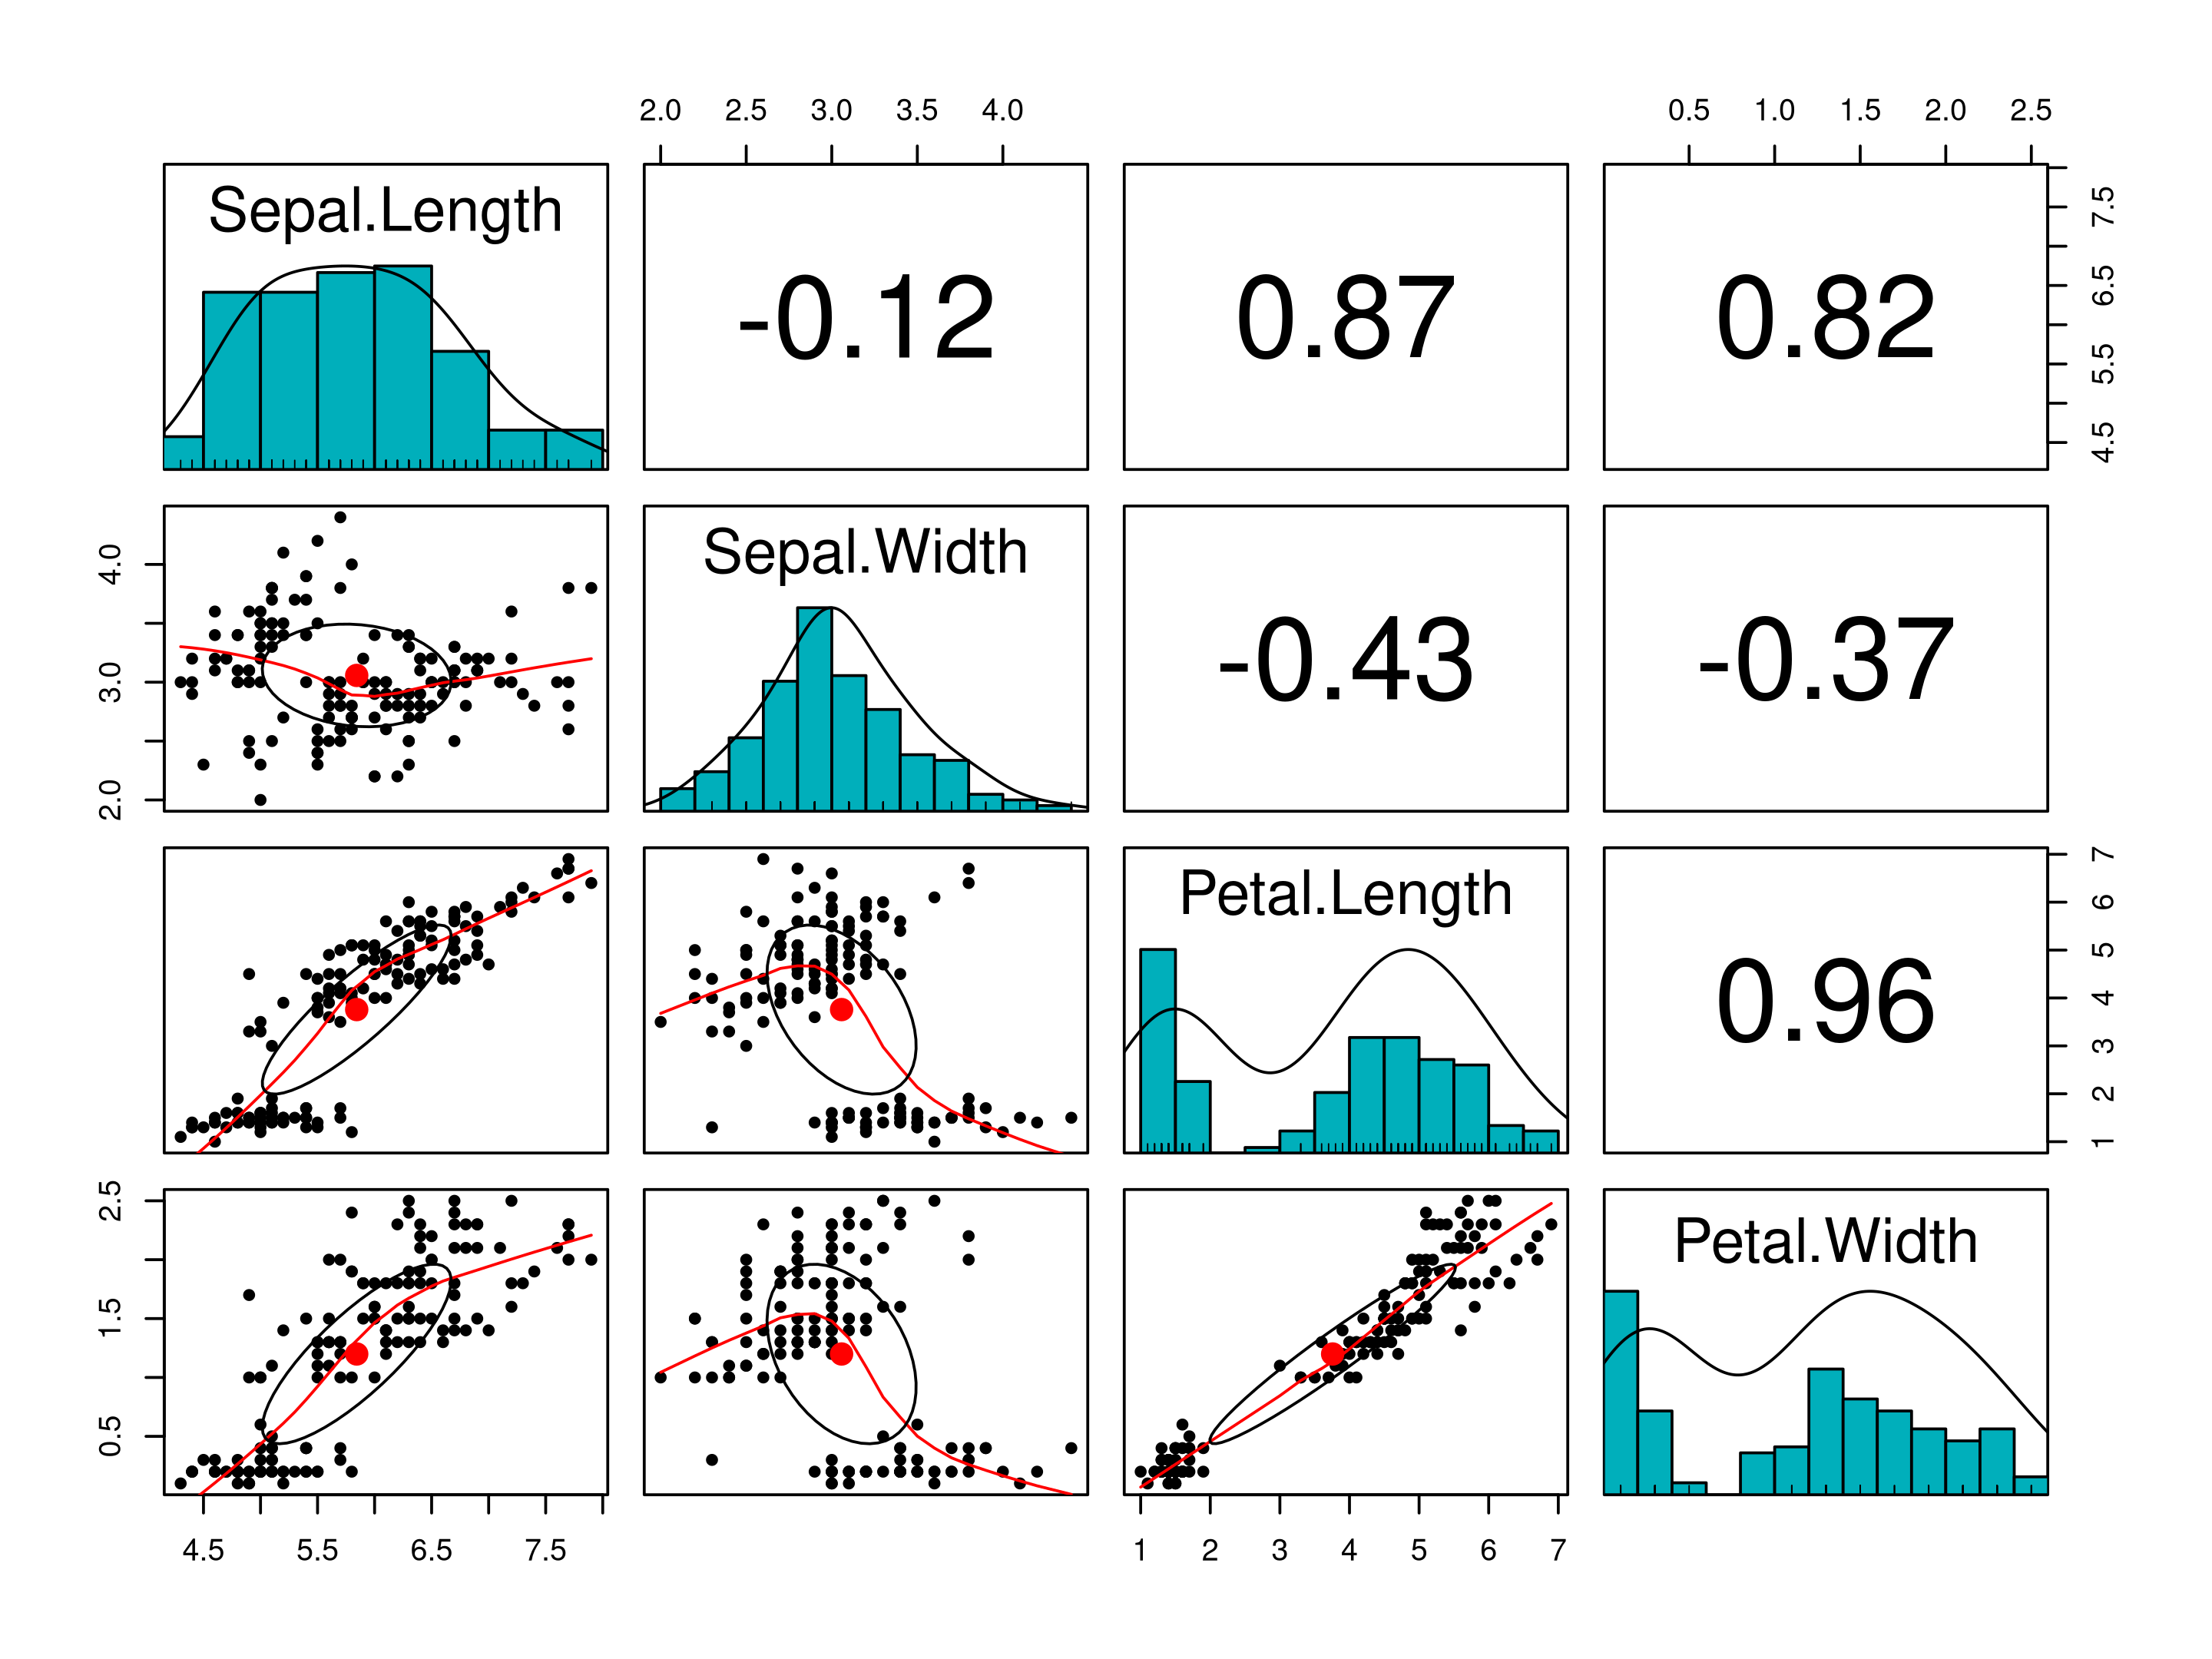
\includegraphics[width=.6\textwidth]{iris}
    \caption{Matrix plot of Iris data}
    \label{fig:mat}
  \end{figure}
\end{frame}

\begin{frame}
  \frametitle{Example (cont.)}\pause
  Let's familiarize ourselves with the classes:\pause
  \begin{figure}[h!]
    \centering
    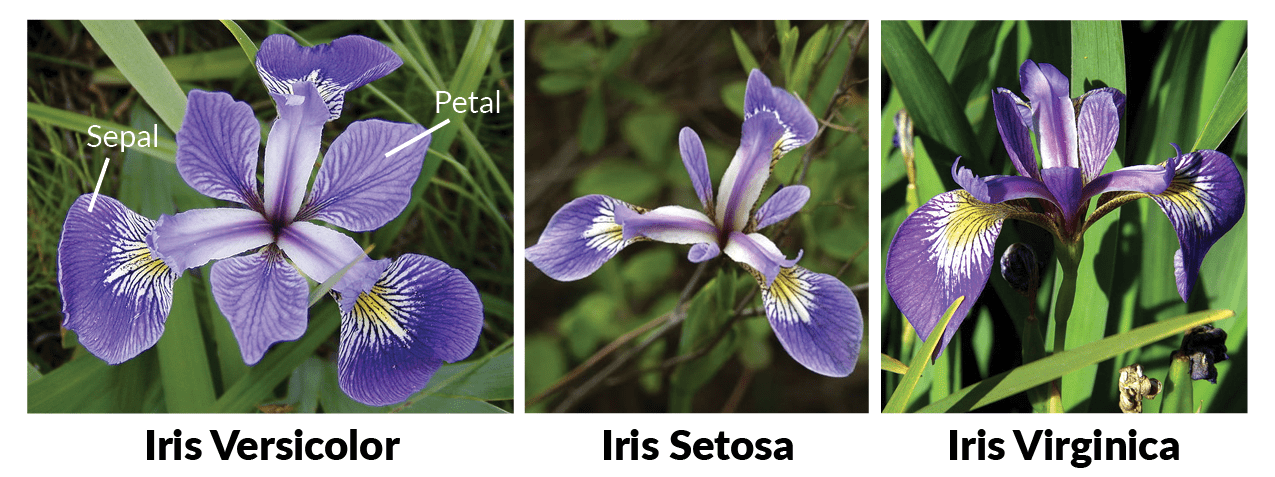
\includegraphics[width=.6\textwidth]{versicolor}
    \caption{3 classes in the Iris data set}
    \label{fig:class}
  \end{figure}
  \pause
  Using the validation set approach with $k=5$, with an 80:20 split, we obtain a prediction accuracy of 93\%.
\end{frame}

\begin{frame}[fragile]
  \frametitle{Example (cont.)}
  \pause
  Implementing LOOCV, we obtain the following output: \pause
  
  \begin{quote}\footnotesize\bl
\begin{verbatim}
k-Nearest Neighbors 

150 samples
  4 predictor
  3 classes: 'setosa', 'versicolor', 'virginica' 

No pre-processing
Resampling: Leave-One-Out Cross-Validation 
Summary of sample sizes: 149, 149, 149, 149, 149, 149, ... 
Resampling results across tuning parameters:

  k  Accuracy   Kappa
  5  0.9666667  0.95 
  7  0.9666667  0.95 
  9  0.9733333  0.96 

Accuracy was used to select the optimal model using the largest value.
The final value used for the model was k = 9.


\end{verbatim}
  \end{quote}
\end{frame}

\begin{frame}[fragile]
  \frametitle{Example: confusion matrices (cont.)}
  Prediction performance with $k=5$:\pause
  
  \begin{quote}\small\rd
\begin{verbatim}
            Reference
Prediction   setosa versicolor virginica
  setosa         10          0         0
  versicolor      0         10         2
  virginica       0          0         8
\end{verbatim}
  \end{quote}
  \pause

  \bigskip
  
  Prediction performance with $k=9$:\pause
  
  \begin{quote}\small\bl
\begin{verbatim}
            Reference
Prediction   setosa versicolor virginica
  setosa         10          0         0
  versicolor      0         10         0
  virginica       0          0        10
\end{verbatim}
  \end{quote}
\end{frame}
\begin{frame}
  \frametitle{$k$-fold cross-validation}
  \pause
  \begin{enumerate}[<+->]
  \item Randomly partition the dataset into  $k$ equally sized groups (or folds)
  \item Taking out the first fold as the validation set, estimate the model on the remaining $k-1$ folds
  \item Compute $MSE_k$ using the validation set:\pause
    \begin{equation}
      MSE_k = \fr1{n_k}\sum_{i'\in k} (y_i - \hat y_i)^2
    \end{equation}
  \item Repeat steps 1--3, successively using the each of the $k-1$ folds as the validation set
  \item Compute the \textbf{\rd $k$-fold CV estimate} of the MSE as:\pause
    \begin{equation}
      \label{eq:15}\rd
      CV_{(k)} = \fr1k \sum_{i=1}^k MSE_i
    \end{equation}
  \end{enumerate}
\end{frame}

\begin{frame}
  \frametitle{$k$-fold CV and LOOCV}
  \pause
  \begin{itemize}[<+->]
  \item LOOCV is a special case of $k$-fold CV \pause
    \note[item]{How is LOOCV a special case of $k$-fold CV?}
    where $k = n$
  \item $k$-fold CV is computationally advantageous, as only $k$ models need to be estimated and $k < n$
  \item The choice of $k$ involves a bias-variance trade-off:
    \begin{itemize}
    \item LOOCV estimates are approximately unbiased but have a higher variance than $k$-fold CV estimates
    \item $k$-fold CV estimates have intermediate bias but have a lower variance since the $k$ models are less correlated than the $n$ models used in LOOCV.
    \item Empirically, $k=5$ and $k=10$ have been shown to produce estimates that have both reasonable bias and variance.
    \end{itemize}
  \end{itemize}
\end{frame}

\begin{frame}
  \frametitle{Cross-validation in classification problems}
  Recall the error rate for a classifier:
  \begin{equation}
    \label{eq:16}
    \Err =  \fr1n \sum_{i=1}^n I( y_{i'} \ne \hat y_{i'}) 
  \end{equation}
  \pause
  The \textbf{\rd LOOCV test error rate} is given by:
  \begin{equation}
    \label{eq:17}\rd
    CV_{(n)} = \fr1n \sum_{i=1}^n \Err_i
  \end{equation}\pause
  where $\Err_i$ is the classification for the $i$th observation:\pause
  \begin{equation}
    \label{eq:18}
    \Err_i = I( y_i \ne \hat y_i) 
  \end{equation}
  Similarly, the \textbf{\rd $k$-fold CV error rate} is given by:
  \begin{equation}
    \label{eq:19}\rd 
    CV_{(k)} = \fr1k \sum_{i=1}^k \Err_i = \fr1k \sum_{i=1}^k \lt(\fr1{n_k} \sum_{i' \in k} I(y_{i'} \ne \hat y_{i'})\rt)
  \end{equation}
\end{frame}

\begin{frame}
  \frametitle{Example: $k$-fold cross validation for model
    selection}
  \pause
  We want to develop a model to predict mileage (\texttt{\bl mpg}) from \texttt{\bl horsepower}.\\ \pause

  \begin{figure}[h!]
    \centering
    \includegraphics<3->[width=.5\textwidth]{mpg-horsepower}
    \caption{MPG vs. horsepower (Auto dataset)}
    \label{fig:auto}
  \end{figure}
  The tuning parameter of interest is the order of the polynomial regression function $\alpha$. %\\ \pause
  
  %$k$-fold cross validation can be used to determine the ``best'' $\alpha$.
\end{frame}


\begin{frame}
  \frametitle{Example: $k$-fold cross validation (cont.)}
  \pause

  We use a 10-fold CV to estimate the MSE for various orders of fit:\pause
  {\footnotesize
  \begin{eqnarray}
    \mathtt{\bl mpg}_1 &=& \beta_0 + \beta_1 \mathtt{\bl horsepower} \\\pause
    \mathtt{\bl mpg}_2 &=& \beta_0 + \beta_1 \mathtt{\bl horsepower} + \beta_2\mathtt{\bl horsepower}^2 \\\pause
    \vdots && \quad\quad \vdots \qquad \qquad \vdots \qquad \qquad \ddots \qquad \qquad \ddots \\\pause
    \mathtt{\bl mpg}_{10} &=& \beta_0 + \beta_1 \mathtt{\bl horsepower} + \cdots + \beta_{10}\mathtt{\bl horsepower}^{10} 
  \end{eqnarray}
}\pause
% \begin{minipage}[t]{.4\linewidth}
  \begin{figure}[h!]
    \centering
    \includegraphics<7->[width=.7\textwidth]{kfold-horsepower}
    \pause
    \caption{$k$-fold test MSE estimate and bias-adjusted $k$-fold CV estimate of MSE.
      While the plot might indicate that a 7th or 8th order fit would be optimal, we must account for  model \textbf{parsimony} and \textbf{interpretability} in making our decision.}
    \label{fig:kfold}
  \end{figure}
% \end{minipage}
% \hfill\pause
% \begin{minipage}[t]{.55\linewidth}

% \end{minipage}
\end{frame}

\begin{frame}
  \frametitle{Example: $k$-fold cross validation (cont.)}\pause
  Based on the plot of the CV estimates of the test MSE, we choose the \textbf{second-order} fit (mpg2) as the best:\pause

  
  \begin{figure}[h!]
    \centering
    \includegraphics<3->[width=.7\textwidth]{mpg-horsepower-fits}
    \caption{$n$th order regression models for mpg on horsepower. The 7th degree model (mpg7) is an overfit.}
    \label{fig:fit}
  \end{figure}
  \pause
  \vspace{-1ex}
  \begin{alertblock}{One-standard-error rule}\pause
    One heuristic used to determine the optimal point on the error vs.\ flexibility curve is to choose the lowest $\alpha$ 
    (most parsimonious model) for which the error is no more than 1 SE above the error of the best model.
  \end{alertblock}
\end{frame}

\begin{frame}
  \frametitle{Cross-validation and predictor selection}
  \begin{minipage}[t]{.47\linewidth}
    \begin{alertblock}{Typical (incorrect) approach}\pause
      \begin{enumerate}[<+->]
      \item Find subset of good predictors that are fairly correlated with class labels/response
      \item Using this chosen subset, build a  classifier/regression model
      \item Use CV to estimate unknown tuning parameters and estimate prediction error of final model
      \end{enumerate}
      With this approach, we obtain test sets that are not independent
    \end{alertblock}
  \end{minipage}\hfill\pause
  \begin{minipage}[t]{.49\linewidth}
    \begin{exampleblock}{Correct approach}\pause
      \begin{enumerate}[<+->]
      \item Randomly partition samples into $k$ folds
      \item For each fold $k$:\pause
        \begin{itemize}[<+->]
        \item Find subset of good predictors that are fairly correlated with class labes/response
        \item Using this predictor subset, build a classifier/regression model on the remaining samples
        \item Use the estimated model to predict observations in fold $k$
        \end{itemize}
      \item Compute/obtain the CV estimate of prediction/test error.
      \end{enumerate}
    \end{exampleblock}    
  \end{minipage}
\end{frame}

\begin{frame}
  \frametitle{Cross-validation and predictor selection (cont.)}
  \pause

  \begin{figure}[h!]
    \centering
    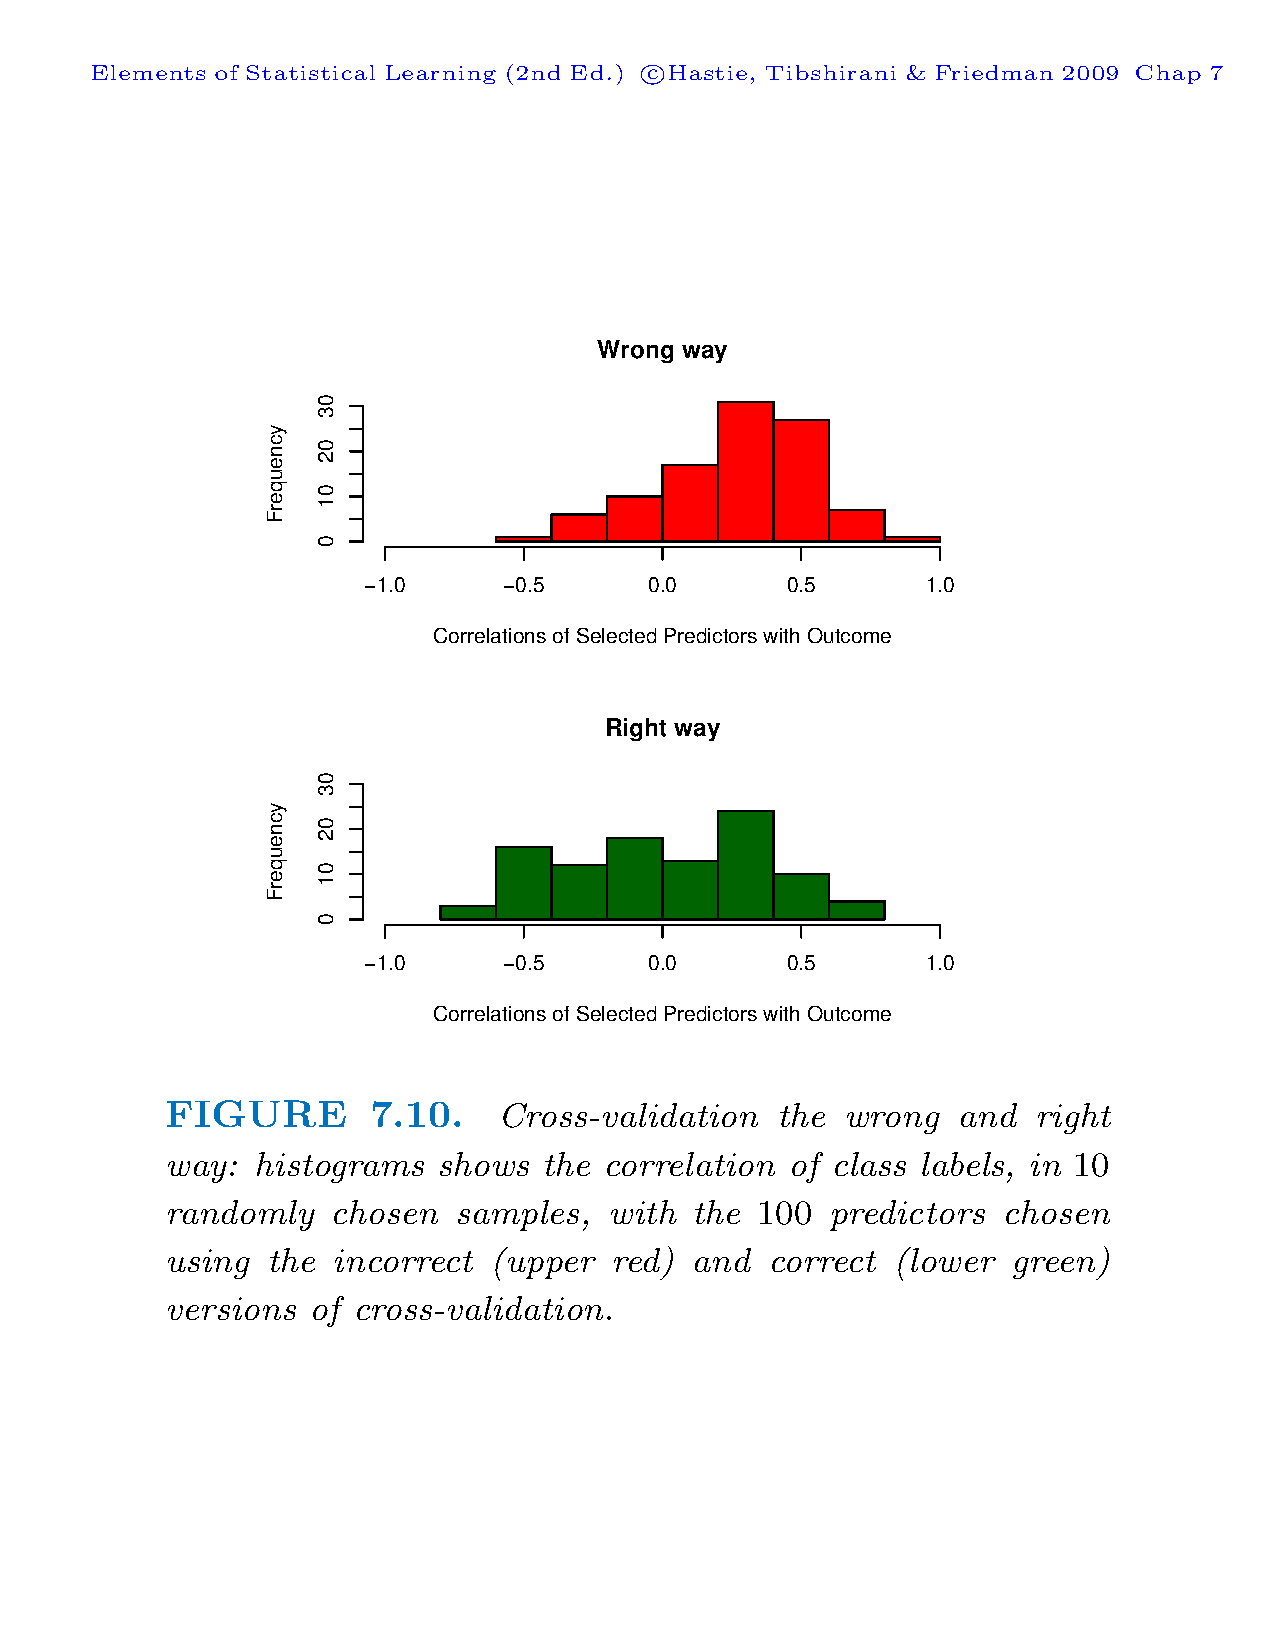
\includegraphics[width=.6\textwidth,trim={2cm 10cm 2cm 5cm},clip]{ESL7-10}
    \caption{{\rd\bf Wrong} (L) and {\gr\bf correct} (R) approach to cross-validation.
      In the wrong approach, the 100 predictors in an random sample of 10 observations have an average correlation of 0.28 w.r.t. the class labels.
      In the correct approach the average correlation is 0.}
    \label{fig:approach}
  \end{figure}
  {\rd Any procedure to remove samples (predictors) should be unsupervised.} %, i.e. without respect to the class labels or response variable.
\end{frame}

\section{The bootstrap}

\begin{frame}
  \frametitle{The bootstrap resampling method}
  \pause

  The bootstrap method\footnote{Introduced by Bradley Efron in \href{https://projecteuclid.org/journals/annals-of-statistics/volume-7/issue-1/Bootstrap-Methods-Another-Look-at-the-Jackknife/10.1214/aos/1176344552.full}{``Bootstrap methods: another look at the jackknife'' (1979)} } (``bootstrapping'') is a resampling technique that estimates the sampling distribution and generates a
  resampled copy of a sample dataset.  \pause

  \begin{itemize}
  \item ``Resampling'' refers to methods for  generates copies of entire datasets (or subsets thereof)
  \item In bootstrapping, the resampling approach used is \textbf{random sampling} (random draws) {\bf  with replacement} 
  \item The resampled dataset (generated copy) is referred to as a {\gr bootstrap sample}
  \item A bootstrap sample of a dataset with $n$ observations (e.g.\ an $n\times p$ matrix) will also have the same dimensions (observations) as the original sample
  \item Bootstrapping is typically performed numerous times (e.g.\ 500, 1000 or 10000) to generate $B$ bootstrap samples
    \begin{itemize}
    \item These resamples can then be used, for example,  to find estimators (known as ``bootstrap estimates'')
    \end{itemize}
  \end{itemize}
\end{frame}


\begin{frame}
  \frametitle{Bootstrap illustration}

  \begin{minipage}{.78\linewidth}
    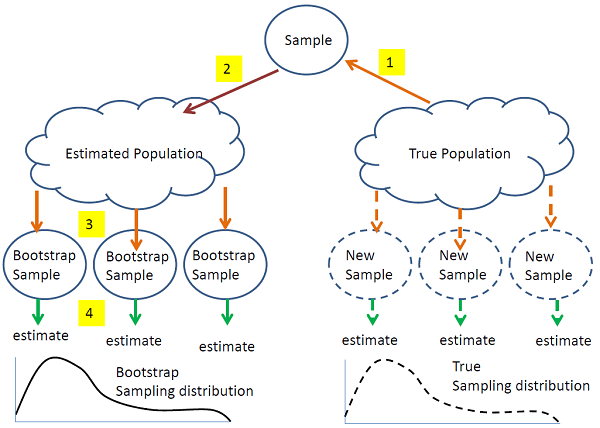
\includegraphics[width=.9\textwidth]{bootstrap-psu}
    
    {\tiny Source: \url{https://online.stat.psu.edu/stat555/node/119/}}\\
    {\footnotesize Solid lines: observed quantities\\
    Dashed lines: unobserved quantities}
  \end{minipage}
  \begin{minipage}{.2\linewidth}\small
    \begin{enumerate}
    \item Sample dataset
    \item Population estimation (implicit)
    \item Bootstrap sample generation (sampling with replacement)
    \item Bootstrap estimates and sampling distribution
    \end{enumerate}
  \end{minipage}
\end{frame}




\begin{frame}
  \frametitle{Generalization of bootstrap approach}
  \textbf{Training set:}\\\pause
  \begin{equation}
    \bm Z = (z_1, z_2, \ldots, z_N),\pause \qquad z_i = (x_i,y_i)
  \end{equation}
  \pause  
  \textbf{Bootstrap samples:}\\\pause
  Generate $B$ bootstrap datasets (e.g. $B=100, B=500, B=1000$) each of size $n$
  by sampling (randomly drawing) from $\bm Z$ \textit{with replacement}:\pause
  \begin{equation}
    \bm Z^{*(r)}, r = 1, \ldots, B
  \end{equation}
  \pause
  
  \textbf{Statistical quantity of interest:}\\\pause
  We define $S(\bm Z)$ as any quantity computed from the dataset $\bm Z$. \\ \pause
  We can estimate any aspect of the distribution of $S(\bm Z)$:\pause
  \begin{align}
    \ol{S}^* &= \fr1B\sum_{r=1}^B S(\bm Z^{*(r)}) \quad \text{sample mean}\\\pause
    \widehat{\text{Var}}[S(\bm Z)] &= \fr{1}{B-1}\sum_{r=1}^B \lt(S(\bm Z^{*(r)}) - \ol{S}^*\rt)^2 \quad \text{variance estimate}
  \end{align}
\end{frame}


\begin{frame}
  \frametitle{Applications of the bootstrap}
  \label{applications}
  \pause
  \begin{itemize}
  \item Generation of dataset samples in ensemble learning methods, such as \pause
    \begin{itemize}
    \item Bagging (``Bootstrap AGGregatING'')\pause
    \item Random forests\pause
    \item Gradient boosting machines\pause
    \end{itemize}
  \item Parameter estimation, e.g.\pause
    \begin{itemize}
    \item Mean, median, mode\pause
    \item Bias, variance\pause
    \item Confidence intervals\pause      
    \end{itemize}
  \item Error estimation\pause
  \item Sampling distribution estimation%\footnote{See \hyperlink{appendix-label}{\beamerbutton{Appendix}}}
  \end{itemize}
\end{frame}

\begin{frame}
  \frametitle{Types of bootstrapping}
  \pause
  \begin{itemize}
  \item \textbf{Nonparametric} (most common and what we consider in this lecture) \pause
    \begin{itemize}
    \item Based on random sampling without replacement\pause
    \item Does not make any assumptions about the distribution of the data\pause
    \end{itemize}
  \item \textbf{Parametric}\pause
    \begin{itemize}
    \item Assumes the underlying distribution of the data is known\pause
    \item Distribution parameters are then estimated from the sample dataset\pause
    \item Samples are then created by generating data from the distributions\pause
    \end{itemize}
  \item \textbf{Semiparametric}\pause
    \begin{itemize}
    \item Combines elements of both parametric and nonparametric approaches\pause
    \item E.g.\ simulates samples based on assumed distributions, then resample residuals/errors and add to simulated
      samples
    \end{itemize}    
  \end{itemize}
\end{frame}

\begin{frame}
  \frametitle{Monte Carlo and bootstrapping}
  \pause

  Monte Carlo methods broadly describe numerical approaches to sampling for statistical inference:\pause
  \begin{itemize}[<+->]
  \item Define uncertainty space (possibility space of variables)
  \item Generate random observations (samples) based on a defined probability distribution (e.g. uniform, Gaussian) over the input space
  \item Perform computation on the samples and aggregate results
  \end{itemize}
  \pause

  \bigskip
  
 {\rd The key difference in [nonparametric] bootstrapping is that we use a given dataset to generate the random samples (i.e.\ the data speak for themselves).} \\ \pause

  \bigskip

  However, parametric bootstrapping can be considered a special case of Monte Carlo.
  
\end{frame}

 \begin{frame}
  \frametitle{The bootstrap method for parameter estimation}
  \pause

  \begin{itemize}[<+->]
  \item General tool for quantifying the uncertainty of a given estimator or statistical method
  %\item Proposed in the 1970's by Brad Efron (see Further Reading)
  \item Example applications:
    \begin{itemize}[<+->]
    \item Estimate standard error of a parameter $\theta$
    \item Estimate bias of a parameter $\hat\theta$: \pause
      \begin{equation}
         \widehat{\text{Bias}}_{\text{B}} = \hat\theta^* - \hat\theta
      \end{equation}
    \pause
    where $\hat\theta^*$ is the average over the bootstrap samples and $\hat\theta$ is the estimate from the original dataset
    \item Construct confidence intervals 
    \end{itemize}
  \end{itemize}
\end{frame}

\begin{frame}
  \frametitle{Estimating statistical parameters from a sample}
  \pause
  \begin{exampleblock}{Example 1}
    \begin{enumerate}[<+->]
    \item What is the ``error'' of the median from a given sample? \pause E.g. how do we compute the bias/variance/MSE of the sample median?
    \item For instance, given a random sample $X_1, \cdots, X_n \sim F$, the $(1-\alpha)100\%$ CI for the population mean is given by:\pause
      \begin{equation}
        \label{eq:11}
        \langle \mu_X \rangle_{1-\alpha} =  \ol{X} \pm z_{\lt(1-\fr\alpha2\rt)}\cdot\fr{\hat\sigma_n}{\sqrt{n}}
      \end{equation} \pause
      How would we obtain a confidence interval (CI) for the population median $x_m$ based on a given sample? 
    \end{enumerate}
  \end{exampleblock}
\end{frame}



\begin{frame}
  \frametitle{Example: Estimating the error of the sample median}
  \pause

  Assume we have a sample of data points: $X_1, \ldots, X_n$. \\ \pause

  Let $M_n = \text{median}\{X_1,\ldots,X_n\}$. \\\pause

  \begin{enumerate}[<+->]
  \item Sample with replacement from these $n$ observations: $X_1^{*(1)}, \ldots, X_n^{*(1)}$
  \item Repeat step 1 to generate a total of $B$ new samples:
    % \begin{tikzpicture}
    %   \draw[rounded rectangle,thick] (0,0) rectangle node[align=center]{
        \begin{align*}
        \text{1st sample:} \quad&  X_1^{*(1)}, \ldots, X_n^{*(1)} \\
        \text{2nd sample:} \quad&  X_1^{*(2)}, \ldots, X_n^{*(2)} \\
        \phantom{\text{1st sample:} } \quad&  \quad \vdots \qquad \vdots \qquad \vdots \\
        \text{$B$th sample:} \quad &  X_1^{*(B)}, \ldots, X_n^{*(B)} 
        \end{align*}
    %   }
    %   (4,8) ;
    % \end{tikzpicture}
  \item For each of these new samples, compute the sample median $M_n^{*(r)}$
  \item From this distribution of bootstrap sample medians, estimate the variance, MSE and CI
  \end{enumerate}
\pause
  The above procedure (generalizable to other statistics) is called the \textbf{\rd empirical bootstrap} or the
  \textbf{\rd nonparameteric bootstrap}.
\end{frame}

\begin{frame}
  \frametitle{Example: Estimating sample median errors (cont.)}
  \pause

  The medians for each sample can be written as:\pause

  \begin{align*}
    M_n^{*(1)} &= \text{median}\{X_1^{*(1)}, \ldots, X_n^{*(1)}\}\\
    M_n^{*(2)} &= \text{median}\{X_1^{*(2)}, \ldots, X_n^{*(2)}\}\\
               &\vdots \\
    M_n^{*(B)} &= \text{median}\{X_1^{*(B)}, \ldots, X_n^{*(B)}\}
  \end{align*}
  \pause
  We can then compute the following estimates:
  \pause

  \bigskip
  \begin{block}{Bootstrap estimate of variance}
    \pause
  \begin{equation}
    \label{eq:13}
    \widehat{\text{Var}}^2_{B}(M_n) = \fr{1}{B-1}\sum_{r=1}^B\lt(M_n^{*(r)} - \ol{M}_B^*\rt)^2
  \end{equation}
  \pause
  where $\ol{M}_B^*$ is the sample mean: \pause
   $ \ol{M}_n^{*} = \fr1B\sum_{r=1}^BM_n^{*(r)}$
\end{block}

\end{frame}

\begin{frame}
  \frametitle{Example: Estimating sample median errors (cont.)}
  \pause

  \begin{block}{Bootstrap estimate of MSE}
    \begin{equation}
      \label{eq:16}
      \widehat{MSE}(M_n) = \fr1B\sum_{r=1}^B\lt(M_n^{*(r)} - M_n\rt)^2
    \end{equation}
  \end{block}
  \pause
  \begin{block}{Bootstrap CI}
    Compute bootstrap differences: $\delta^* = \hat M_n^* - \hat M_n $; sort them and find the percentiles (critical values) $\delta^*$:
    \begin{equation}
      \label{eq:17}
      \langle M_n \rangle_{1-\alpha} = M_n \pm  \delta_{1-\alpha}^* 
    \end{equation}
  \end{block}
  \pause

  \begin{alertblock}{Notes}
    \begin{itemize}[<+->]\footnotesize
    \item The CDF of the bootstrap statistic $M_n^{*(r)}$ tends toward the true CDF as $n\to\infty$
      because the observations in the bootstrap samples are independent and identically distributed (IID).
    \item \textbf{Parametric} bootstrapping can be done if the bootstrap samples have a known underlying process, e.g. Gaussian, exponential, etc.
    \end{itemize}
  \end{alertblock}
\end{frame}
\begin{frame}
  \frametitle{Example: Bootstrap estimates of mean and variance}\pause
  Using the \texttt{\bl faithful} dataset, we demonstrate how the bootstrap can be used to quantify the uncertainty of the mean and variance of the elapsed time between successive eruptions.

  \pause

  \begin{center}
    \includegraphics<3->[width=.6\textwidth]{waiting}
  \end{center}

  \pause

    (See \texttt{M3b-Bootstrapping-R.ipynb} for the solution.)
\end{frame}



% \begin{frame}
%   \frametitle{Example 4: Bootstrapping for trimmed mean estimates}
%   \pause

%   In the L1 German vocabulary test (WST), we want to compute the sample mean but disregarding the lowest 10\% scores (this is a trimmed mean).
%   From the sample, this value is 32.7. But how do we compute a confidence interval?

%   \begin{center}
%     \includegraphics<3->[width=.6\textwidth]{boot3}
%   \end{center}
% \end{frame}






\begin{frame}
  \frametitle{$k$-fold CV  vs. bootstrapping for prediction error}
  \pause
  We define \textit{overlap} as the fraction of observations in a training set relative to the validation set.\pause
  
  \begin{itemize}[<+->]
  \item In $k$-fold CV, each validation fold is distinct from the other training folds---\pause \textbf{no overlap} between training and validation samples:\pause
    \begin{enumerate}[<+->]
    \item Fit model with $n- \fr nk$ observations (training set)
    \item Evaluate performance on remaining $\fr nk$ observations (validation set)
    \item Repeat steps 1 and 2 for the $k$ different folds and then find the expected prediction error
      (and its standard deviation)
    \end{enumerate}
  \end{itemize}
  \pause

  \begin{exampleblock}{Question}
    Each bootstrap sample $\bm Z^{*(r)}$ has considerable overlap with the original dataset $\bm Z$.\\
    \pause

    \bigskip
      
    What is the value of this overlap?
  \end{exampleblock}
\end{frame}




\section{Outlook}

\begin{frame}
  \frametitle{Reading assignments}

  \begin{itemize}
  \item \textbf{PMLI} 4 (you may skim/skip the sections with asterisks; but focus on those topics covered in the lectures).
    \begin{itemize}
      \item CV is introduced within the context of regularization (4.5); still good to read entire section as we will return to these concepts later
    \item Section 4.7.6 Bias-variance tradeoff (which we did not cover in class)
    \end{itemize}
  \item \textbf{ESL} 7.1--7.7, 7.10--12

  \end{itemize}
\end{frame}

% \begin{frame}
%   \frametitle{Introduction to Python/JupyterLab/R}
%   \pause

%   More will be said on this next lecture.

%   \pause

%   You can find a helpful tutorial at \url{https://cs231n.github.io/python-numpy-tutorial/#jupyter-and-colab-notebooks}.
% \end{frame}

\appendix\addtocounter{part}{-1}

% \section{Appendix: ECDF}
% \label{appendix-label}
% \begin{frame}
%   \frametitle{Empirical distribution function (ECDF)}
%   \pause

%   Given $n$ independent observations $X = (X_1, \ldots, X_n)$, where $X_i \sim F$ (where $F$ is the unknown true distribution function).\pause

%   \bigskip
  
%   The \textbf{\gr empirical (or nonparametric) distribution function} is defined as:\pause

%   \begin{equation}\gr
%     \widehat F(x) = \fr{\#(X_1 \le x, \ldots, X_n \le x)}{n}\pause = \fr1n\sum_{i=1}^n I(X_i\le x)
%   \end{equation}
%   \pause
  
%   This is a discrete distribution that assigns a probability of $\fr1n$ at each data point $X_i$.\pause
%   \bigskip

%   A standard result is that $\widehat F \to F$ as $n\to \infty$.

%   \hyperlink{applications}{\beamerbutton{Back}}
  
% \end{frame}



\section{Appendix}
\begin{frame}
  \frametitle{Example: Estimating the SE of a composite variable}
  Given a variable $\al$ that minimizes risk in a portfolio of two investments, its estimate is given by:\pause
  \begin{equation}
    \label{eq:18}
    \hat\al = \fr{\hat\si_Y^2 - \hat\si_{XY}}{\si_{X}^2 + \si_Y^2 - 2\hat\si_{XY}}
  \end{equation}
  \pause
  How would we then estimate the standard error of $\hat\al$, $SE(\hat\al)$? \pause
  
  \begin{exampleblock}{}
  In practice, it is impossible to estimate the standard error of $\hat\alpha$, as we cannot generate brand new samples from the original population.\\ \pause

  Thus, we use the bootstrap to perform the estimate by generating $B$ bootstrap samples and computing the $SE$ estimate
  by:\pause
  
  \begin{equation}
    \label{eq:10}
    SE_{B}(\hat\al) = \sqrt{\fr{1}{B-1}\sum_{r=1}^B\lt( \hat\alpha^{*r} - {\bl \fr1B\sum_{r'=1}^B\hat\al^{*r'}} \rt)^2 }
  \end{equation}
  \pause
  Note that the term in blue is the \textbf{\bl bootstrap mean estimate of $\hat\al$}.
\end{exampleblock}

\end{frame}


 
\begin{frame}
  \frametitle{Bootstrap estimation of prediction error}
  Assume we generate $B$ bootstrap samples from a given data set.\\\pause

  \bigskip

  Let the predicted value at point $x_i$ from a model fitted to the $r$th bootstrap dataset be  $\hat f^{*(r)}(x_i)$. \\ \pause

  \bigskip
  
  Then, the prediction error could be estimated as: \pause
  \begin{equation}
    \widehat{\Err}_{\text{boot}} = \fr1B\fr1n\sum_{r=1}^B\sum_{i=1}^n L(y_i,\hat f^{*(r)}(x_i))
  \end{equation}

  \begin{alertblock}{Problems with this approach}\pause
    \begin{itemize}[<+->]
    \item Bootstrap datasets act as training samples, while original training set acts as test sample
    \item Thus there is overlap of observations between the samples
    \item This would lead to an underestimation of the true error (overfitting of predictions)
    \end{itemize}
  \end{alertblock}
\end{frame}


\begin{frame}
  \frametitle{Overlap of observations in bootstrap sample}
  \pause
  For the first  random draw $z_1^{*(r)}$ to populate a bootstrap sample $\bm Z^{*(r)}$, \pause
  the probability that observation $i$ will be drawn is:\pause
  \begin{equation}\bl
     \Pr\{\text{observation } i \text{ is drawn}\} = \fr 1n
  \end{equation}
  \pause
  Then the probability that observation $i$ will \textit{not} be drawn is:\pause
  \begin{equation}\rd
    \Pr\{\text{observation } i \text{ not drawn}\} = 1 - \fr{1}{n}
  \end{equation}
  \pause
  Therefore, the probability that observation $i$ will \textit{not} be selected in any of the $n$ bootstrap sample random draws is:\pause
  \begin{equation}\rd 
    \Pr\{\text{observation } i \notin \text{ bootstrap sample } \bm Z^{*(r)} \}
    \pause  = \lt(1 - \fr1n\rt)^n
  \end{equation}
\end{frame}

%https://math.stackexchange.com/questions/1031741/binomial-expansion-of-1-xn
\begin{frame}
  \frametitle{Overlap of observations in bootstrap sample (cont.)}
  \pause

  Recall the \textbf{\bl Maclaurin Series} (Taylor expansion about 0):\pause
  \begin{equation}\bl
    f(x) = f(0) + f'(0)\cdot x +\fr{ f''(0)}{2!}\cdot  x^2 + \fr{ f^{(3)}(0)}{3!}\cdot  x^3 \pause =
    \sum_{n=1}^\infty \fr{ f^{(n)}(0)}{n!} \cdot x^n
  \end{equation}
  \pause
  Applying this to $e^{-1}$, we obtain an alternating series:\pause
  \begin{equation}
    e^{-1} = \pause 1 - 1 + \fr{1}{2!} - \fr{1}{3!} + \cdots
  \end{equation}
  \pause
  Also recall the \textbf{\gr binomial expansion}:\pause
  \begin{equation}\gr
    (1-x)^n = \pause \sum_{k=0}^n {n \choose k}1^{n-k}(-x)^k = \pause
    1 - nx + \fr{n(n-1)}{2!}\cdot x^2 - \fr{n(n-1)(n-2)}{3!}\cdot x^3 + \cdots
  \end{equation}
  \pause
  If we let $x = \fr 1n$, then:\pause
  \begin{equation}
    \lt(1-\fr1n\rt)^n = 1 - 1 + \fr{n-1}{2 \cdot n} -\pause \fr{(n-1)(n-2)}{3!\cdot n^2} \pause \approx e^{-1}
  \end{equation}

\end{frame}

\begin{frame}
  \frametitle{Overlap of observations in bootstrap sample (cont.)}
  \pause
  We can then approximate the probability that an observation will not be in a given bootstrap sample as:\pause
  \begin{equation}\rd
    \Pr\{\text{observation } i \notin \text{ bootstrap sample } \bm Z^{*(r)} \}
    \pause  = \lt(1 - \fr1n\rt)^n  \pause
    \approx e^{-1} = 0.368
  \end{equation}
  \pause
  Finally we can approximate the overlap as follows:\pause
  \begin{eqnarray*}
     \Pr\{\text{observation } i \in \text{ bootstrap sample } \bm Z^{*(r)} \} \pause &=&
    1 -  {\pl \lt(1 - \fr1n\rt)^n}\\
    \pause &\approx& 1 - {\pl 0.368}\\  \pause
    & =& 0.632
   \end{eqnarray*}
\end{frame}
\begin{frame}
  \frametitle{Example: Bootstrap overfitting}\pause
  Given a binary classification problem with the same number of observations per class (equal priors); predictors and class labels are independent. 
  \begin{enumerate}[a]
  \item What is the true error rate? \pause 
  \item Find the bootstrap estimate of the error rate
  \end{enumerate}
  \pause

  \begin{exampleblock}{Example 4: Solution}
    \pause
    \begin{enumerate}[\bf a]
    \item The true error rate is 0.5 ($\pi_{1} = \pi_{2} = 0.5$) \pause

    \item The bootstrap error estimate is given by:\pause
    \begin{equation}
         \widehat{\Err}_{\text{boot}} = \fr1B\fr1n\sum_{r=1}^B\sum_{i=1}^n L(y_i,\hat f^{*(r)}(x_i))
       \end{equation}
       \pause
  Contributions (loss function evaluation) to the bootstrap estimate $ \widehat{\Err}_{\text{boot}} $
  will be 1 if the $i$th observation \textit{does not appear} the bootstrap sample $ \bm Z^{*(r)}$. \\
  \pause
  This occurs 36.8\% of the time, as we just derived. \pause
  Since there is a 50-50 chance of assignment to either class, \pause
  the \textbf{\rd expected training error estimate} is given by:\pause
  \begin{equation*}\rd
    E(\widehat{\Err}_{\text{boot}}) = \pause 0.5 \times 0.368 = \pause 0.184
  \end{equation*}
    \end{enumerate}
 
\end{exampleblock}

  
  \note[item]{Question: what is wrong with this estimate?}

\end{frame}

\begin{frame}
  \frametitle{Correcting the bootstrap overfit}
  \pause

  To correct the overfitting, we can compute the \textbf{\bl leave-one-out bootstrap
    estimate}:\pause
  \begin{equation}\bl
    \widehat{\Err}^{(1)} = \fr1n\sum_{i=1}^n \fr{1}{|C^{-i}|}\sum_{r \in C^{-1}}L(y_i,\hat f^{*(r)}(x_i))
  \end{equation}
  \pause
  where $C^{-i}$ is the set of indices of the bootstrap samples  $\bm Z^{*(r)}$ that do not contain
  the $i$th observation, \pause and $|C^{-1}|$ is the number of these samples. \pause

  \bigskip
  \begin{itemize}[<+->]
  \item Average number of distinct observations in each bootstrap sample $\approx 0.632n$.
  \item $\widehat{\Err}^{(1)}$ is biased as a significant portion of the data are not used in training
  \item This bias can be corrected using the \textbf{\pl .632 estimator}:\pause
    \begin{equation}\pl
      \widehat{\Err}^{(.632)} = \pause .368\cdot\ol\err + \pause .632\cdot\widehat{\Err}^{(1)}
    \end{equation}
    \pause
    where $\ol\err$ is the training error (average loss over the training sample)
  \end{itemize}
\end{frame}

\begin{frame}
  \frametitle{Correcting the bootstrap overfit (cont.)}
  \pause

  \begin{itemize}
  \item The .632 estimator works well in many situations
  \item However, it can still fail to correctly approximate the true error
  \item In the binary case of independent classes, equal priors with 1-nearest neighbor classifier:\pause
    \begin{eqnarray*}
      \ol\err &=& 0 \\\pause
      \widehat\Err^{(1)} &=& 0.5 \\\pause
      \implies\quad \pause \widehat\Err^{0.632} &=& 0.368(0) + 0.632(0.5) \pause = 0.316
    \end{eqnarray*}\pause
    which is an improvement over 0.184 but still much lower than 0.5
  \end{itemize}
\end{frame}


\end{document}

%%% Local Variables:
%%% mode: latex
%%% TeX-master: t
%%% End:
